\section{MK5i Swerve Motor Module Assembly}
\resetassemblysteps

\begin{partsbox}
\begin{minipage}[t]{\linewidth}
\vspace{0pt}
\begin{itemize}
    \item 8 \hyperref[sec:motor-assembly]{Assembled Motors}
    \item 4 \href{https://www.swervedrivespecialties.com/collections/all/products/mk5i-swerve-module?variant=51829284602157}{MK5i Swerve Module Kits}
    \item 4 \href{https://andymark.com/products/cancoder-magnetic-encoder?variant=44493487145132}{CANcoder Magnetic Encoders}
\end{itemize}
\end{minipage}
\end{partsbox}

These modules come mostly assembled, but the motors and encoders need to be installed and the gear ratio may need adjusting.

\assemblystep{Change Gear Ratio}

First, looking at the top surface of the module, lightly loosen the
right hand screw on the metallic plate. The left hand screw will need to
then be loosened until it can be lifted and pulled down to gear ratio 1.

\begin{figure}[H]
\centering
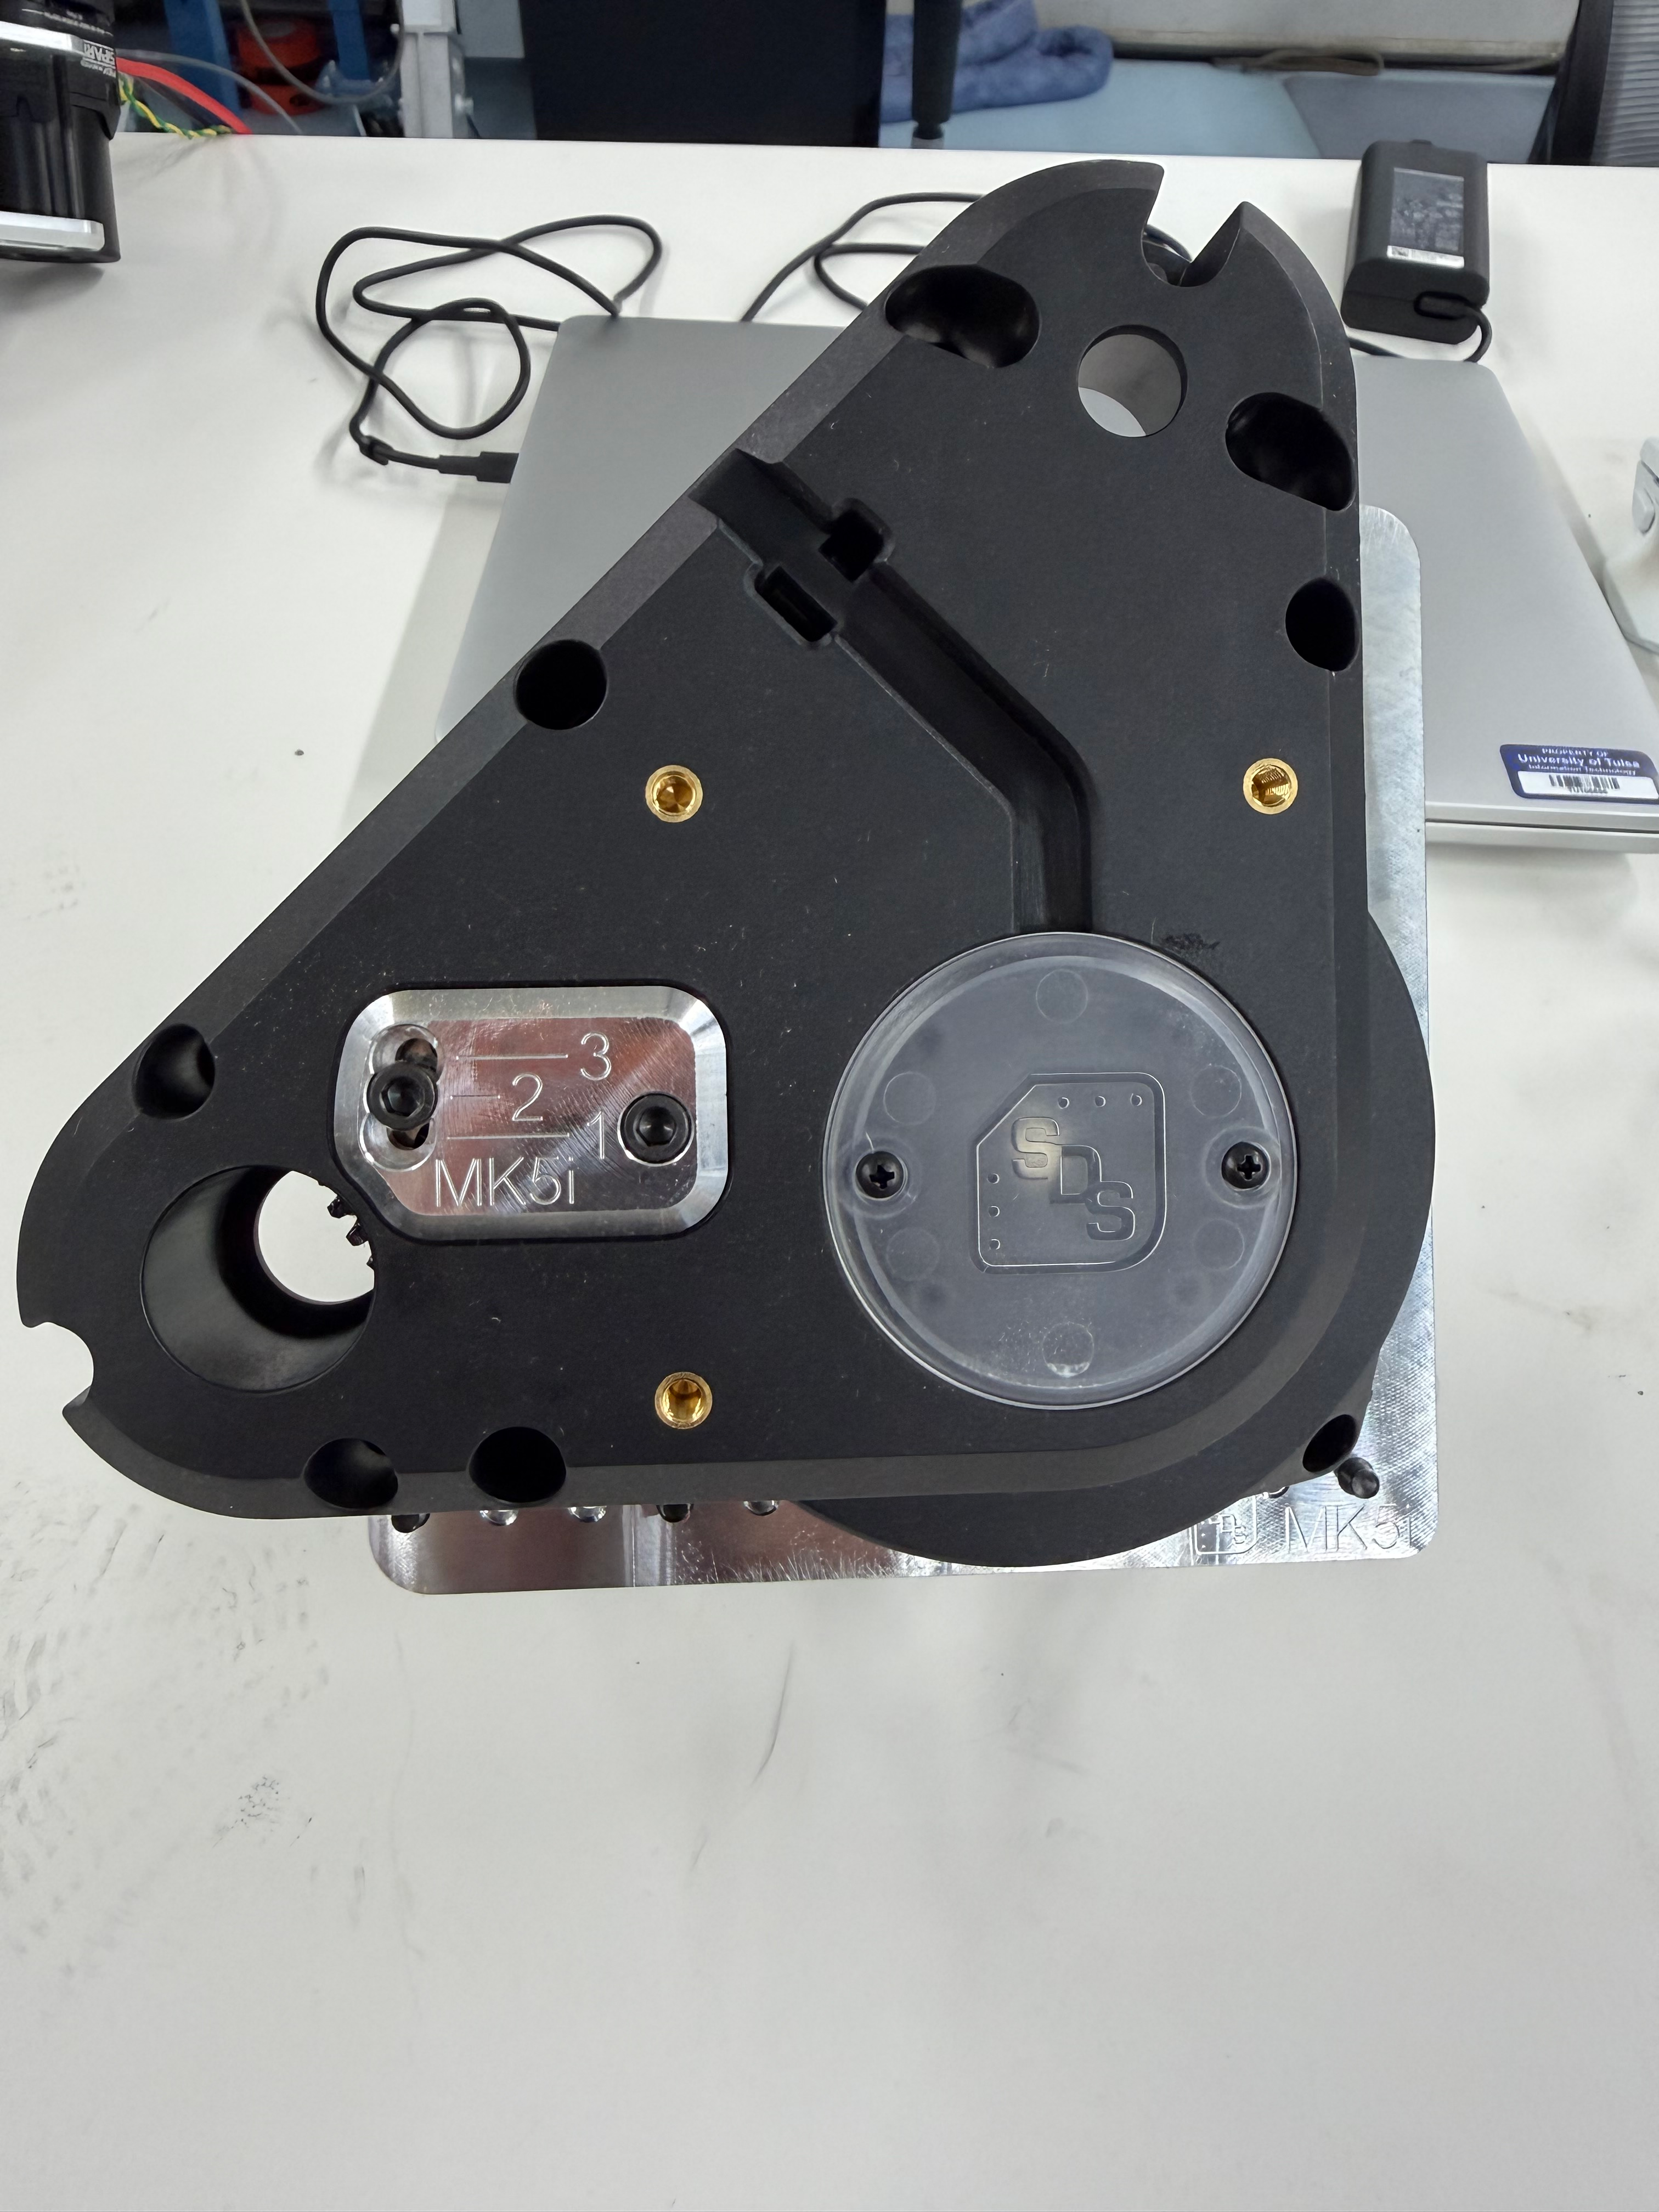
\includegraphics[width=0.5\textwidth]{media/image8.png}
\caption{Top of Swerve Module before adjusting gear ratio, default setting is on 2.}
\end{figure}

\assemblystep{Steer Motor Installation}
The first motor will need the hardware kit containing the 1mm thick
washer (or shim), 14T pinion gear, 2mm machine key, and 8mm retaining
ring.

\begin{figure}[H]
\centering
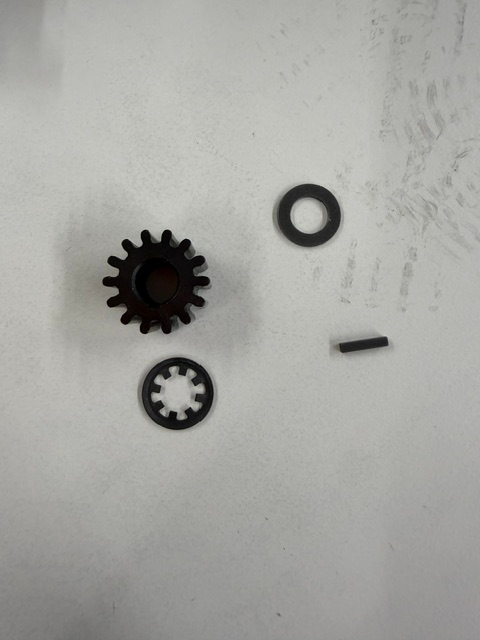
\includegraphics[width=0.5\textwidth,angle=90,origin=c]{media/image9.png}
\caption{Steer motor hardware kit: shim washer, 14T pinion gear, machine
key, and 8mm retaining ring.}
\end{figure}

\clearpage
Place the washer on the motor shaft, then install the machine key into
the groove on the shaft. Slide the pinion gear onto the shaft, making
sure to align the key slot on the inside of the gear with the key. To
install the retaining ring, a long ratchet socket and a rubber mallet
can be used.

\begin{figure}[H]
\centering
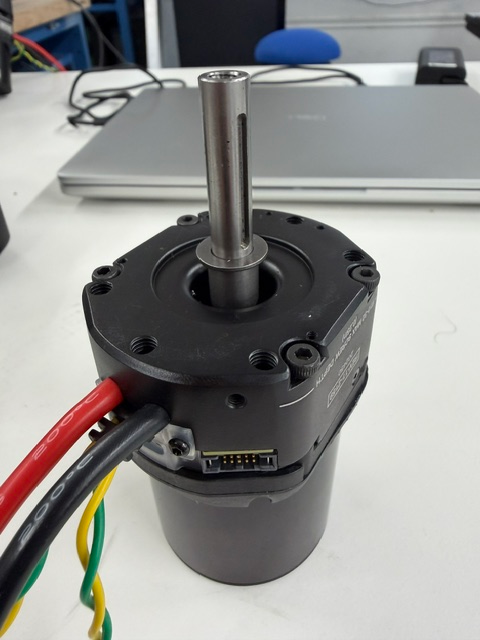
\includegraphics[width=0.31\textwidth]{media/image10.png}
\hfill
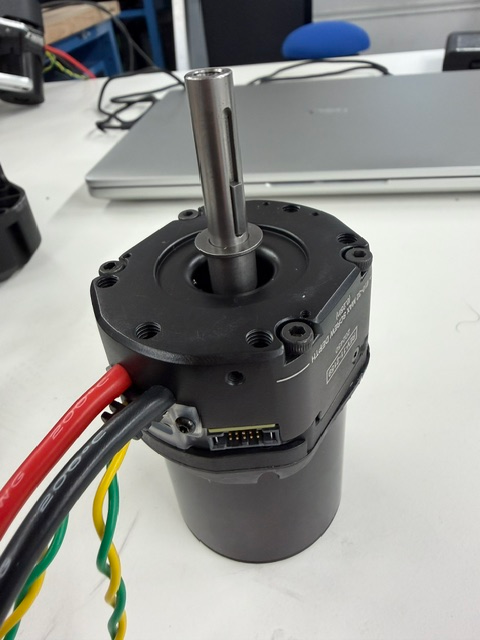
\includegraphics[width=0.31\textwidth]{media/image11.png}
\hfill
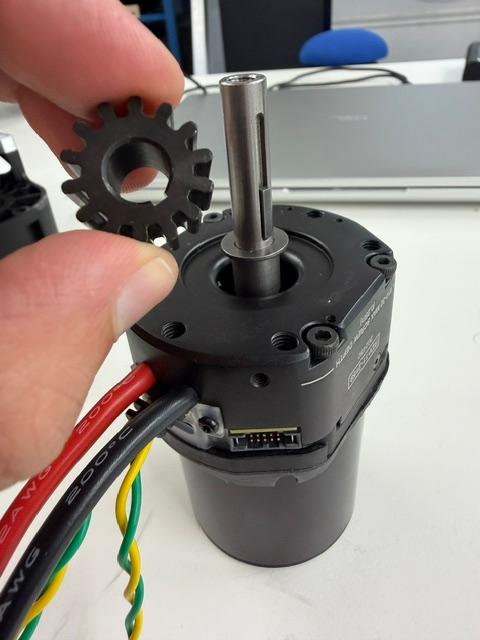
\includegraphics[width=0.31\textwidth]{media/image12.png}

\vspace{0.4cm}
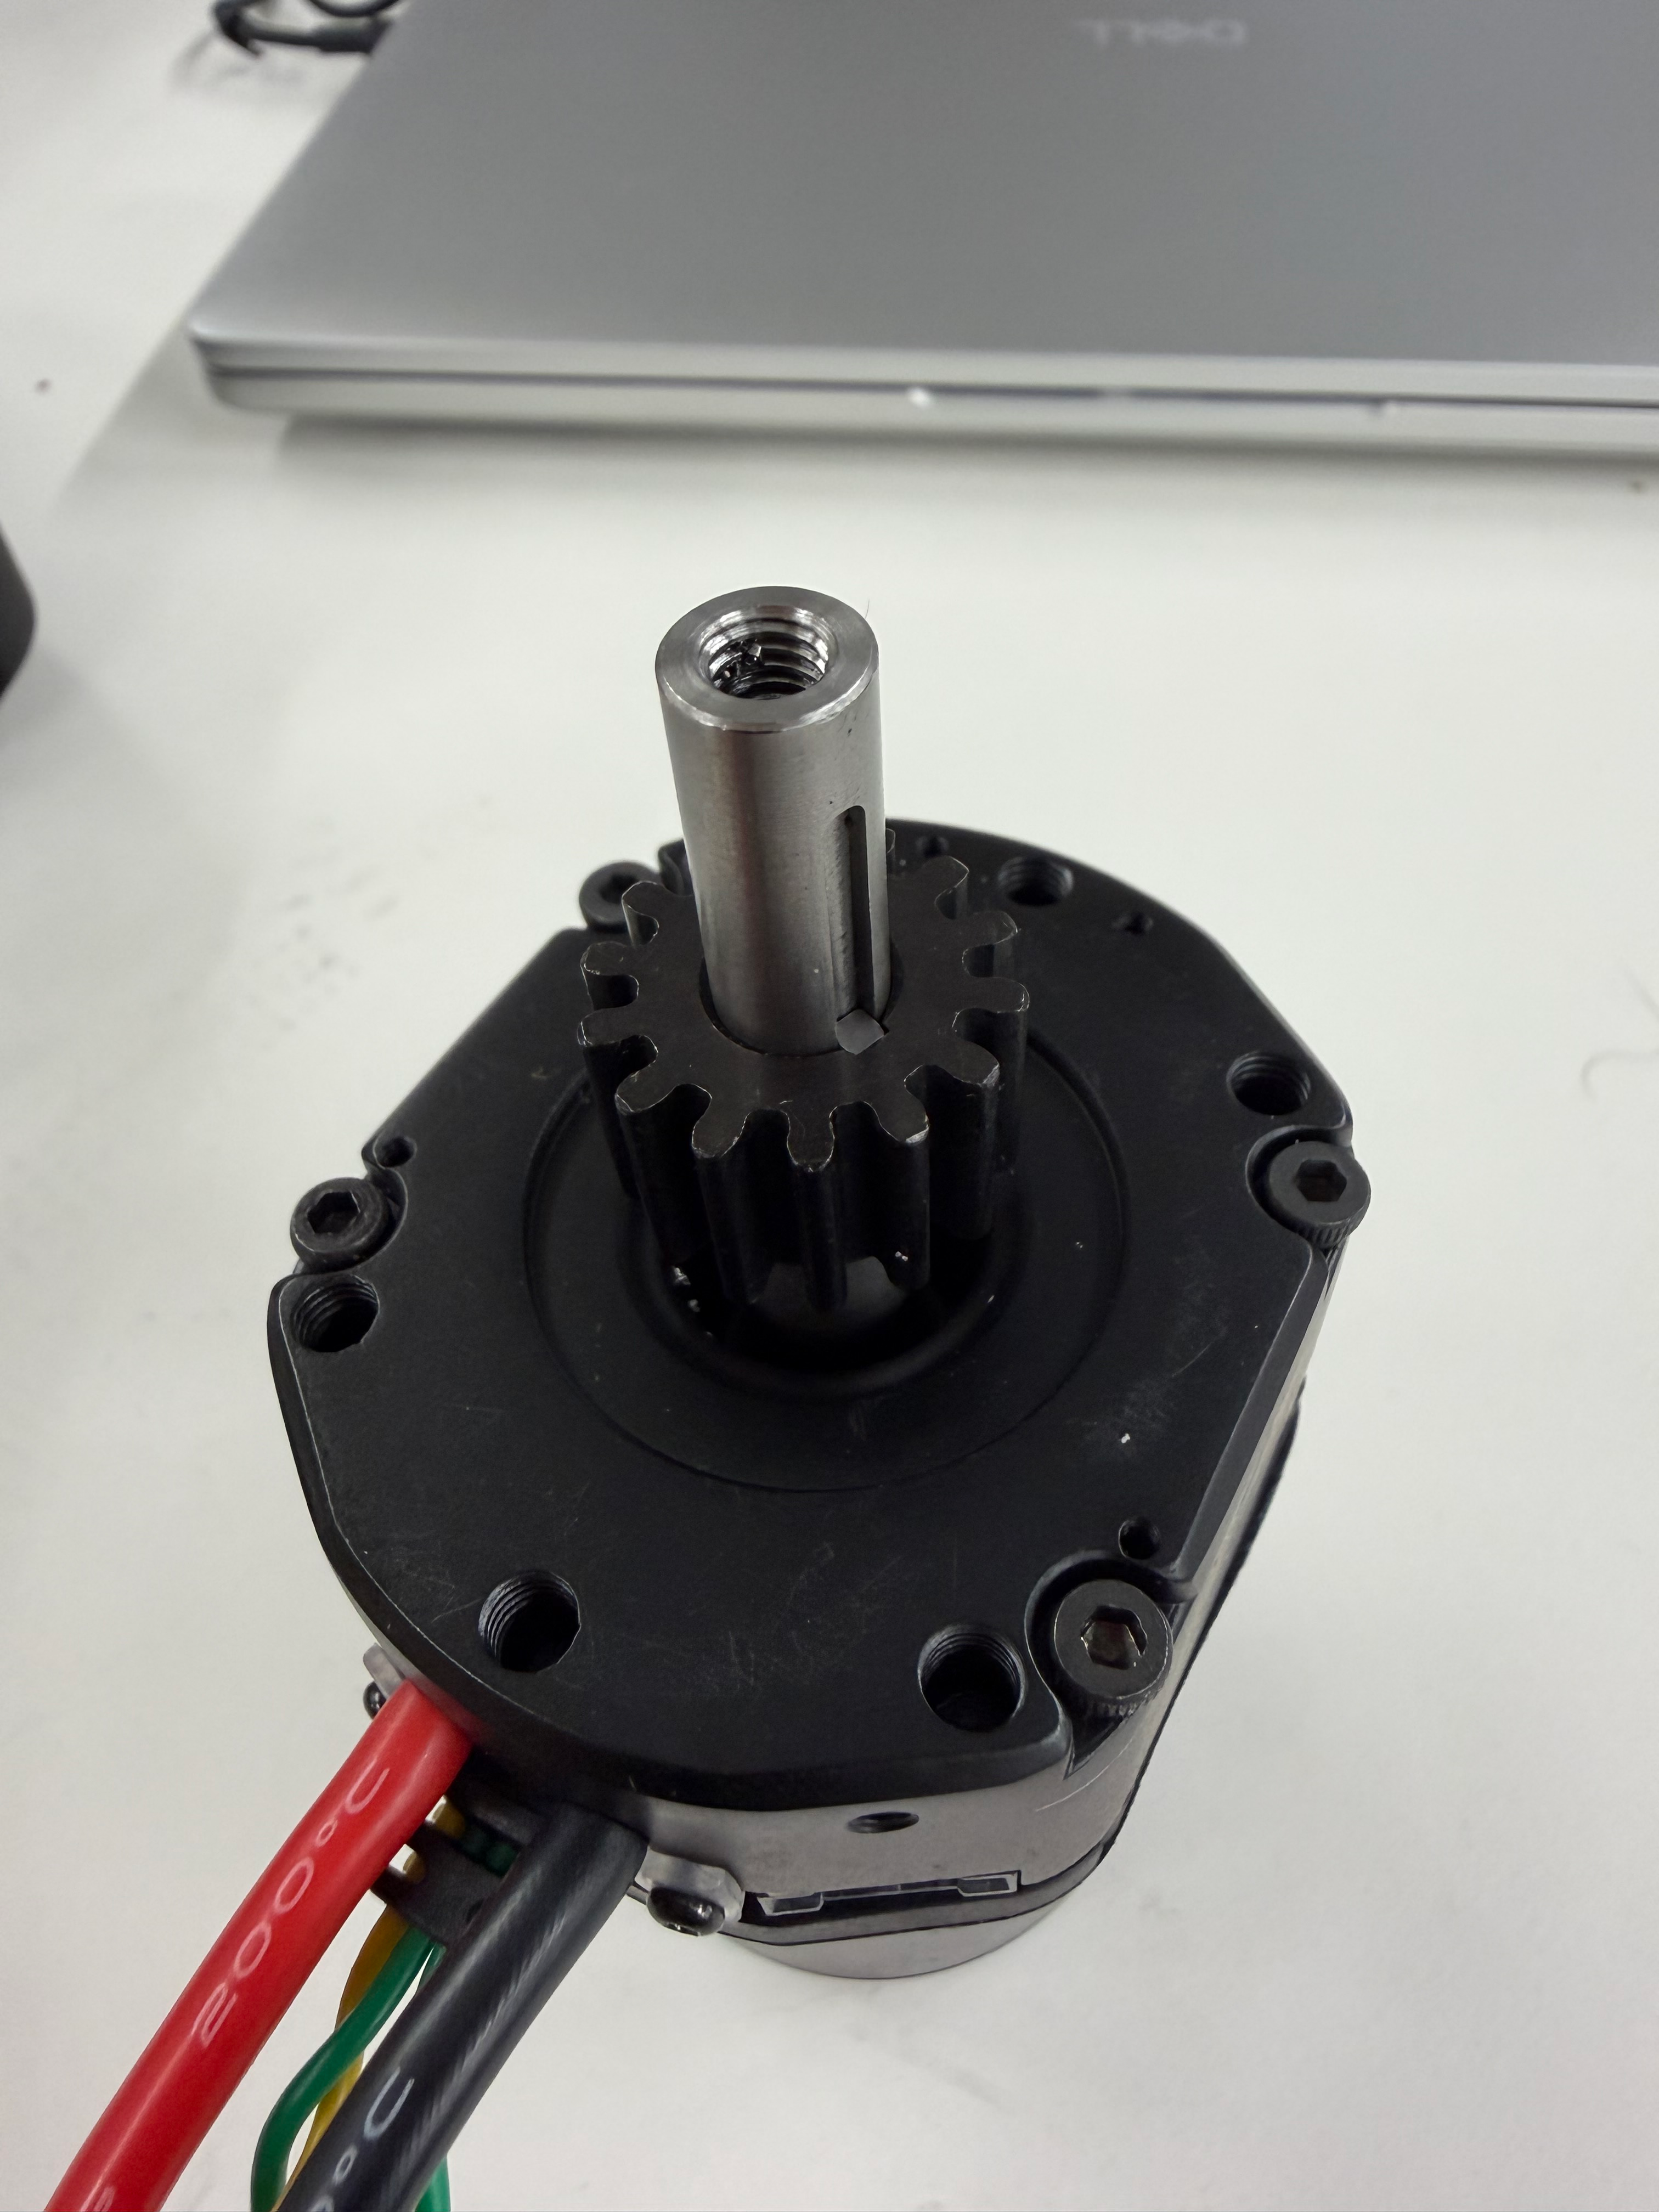
\includegraphics[width=0.31\textwidth]{media/image13.png}
\hfill
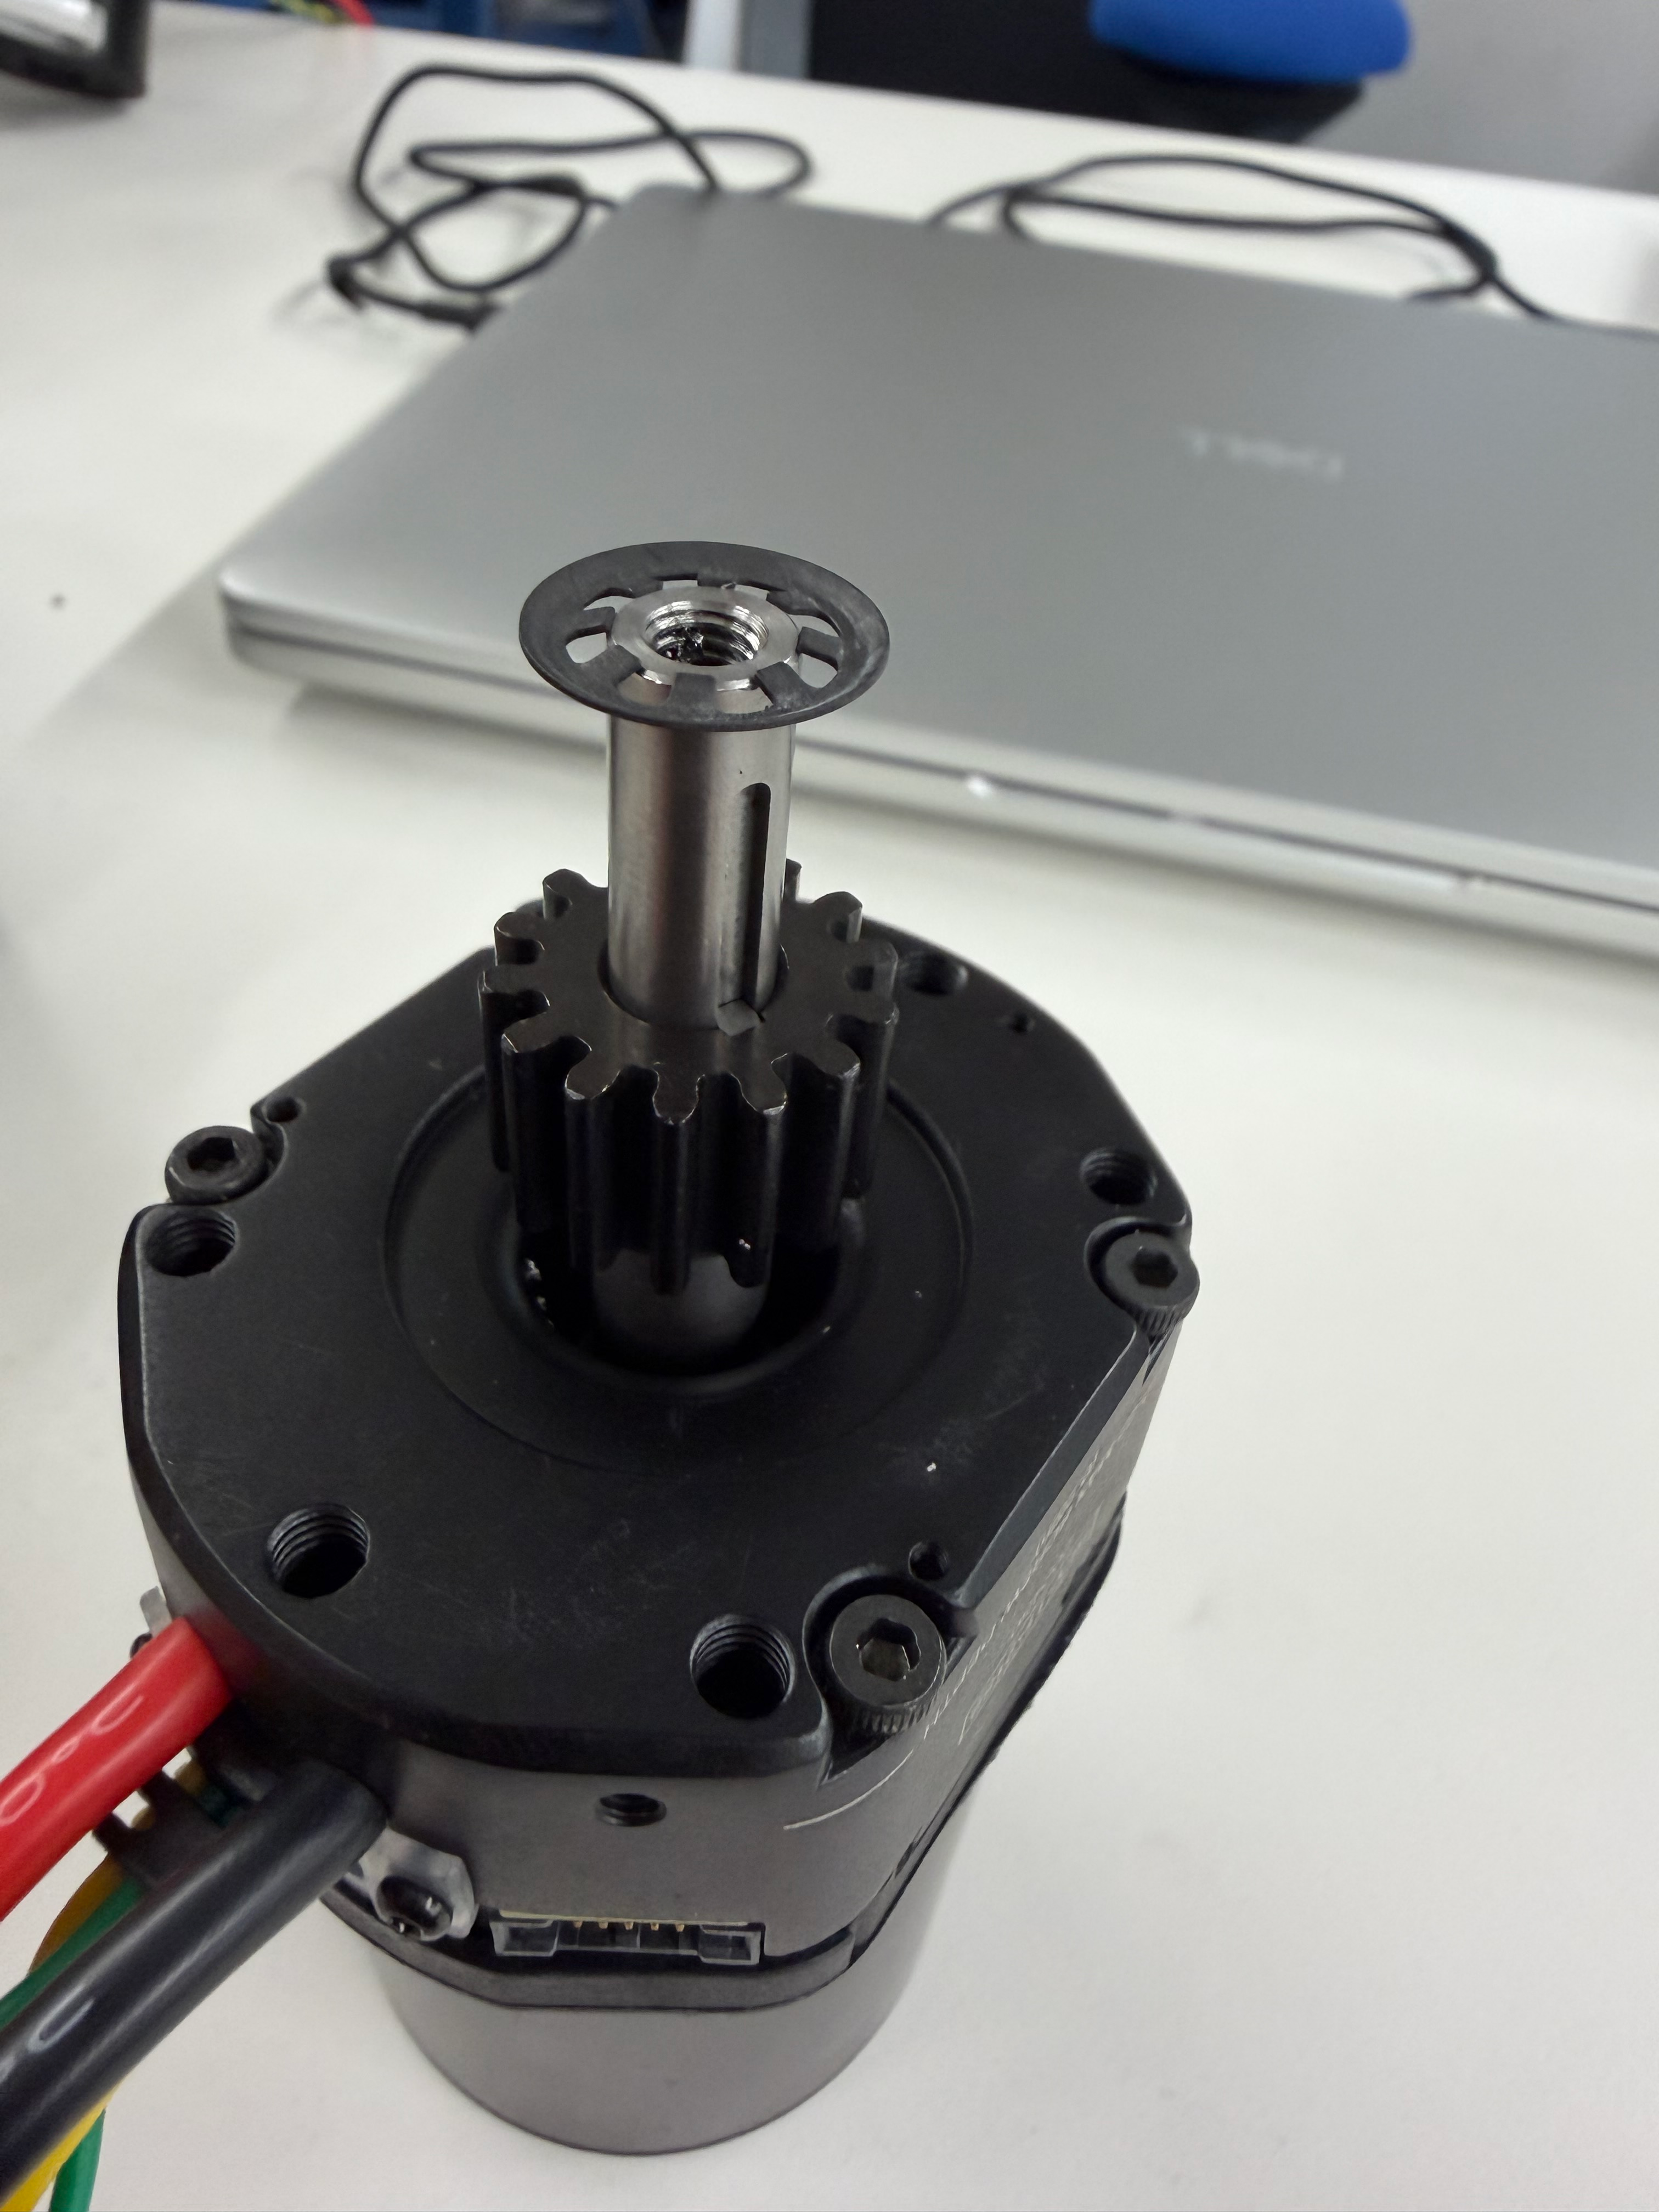
\includegraphics[width=0.31\textwidth]{media/image14.png}
\hfill
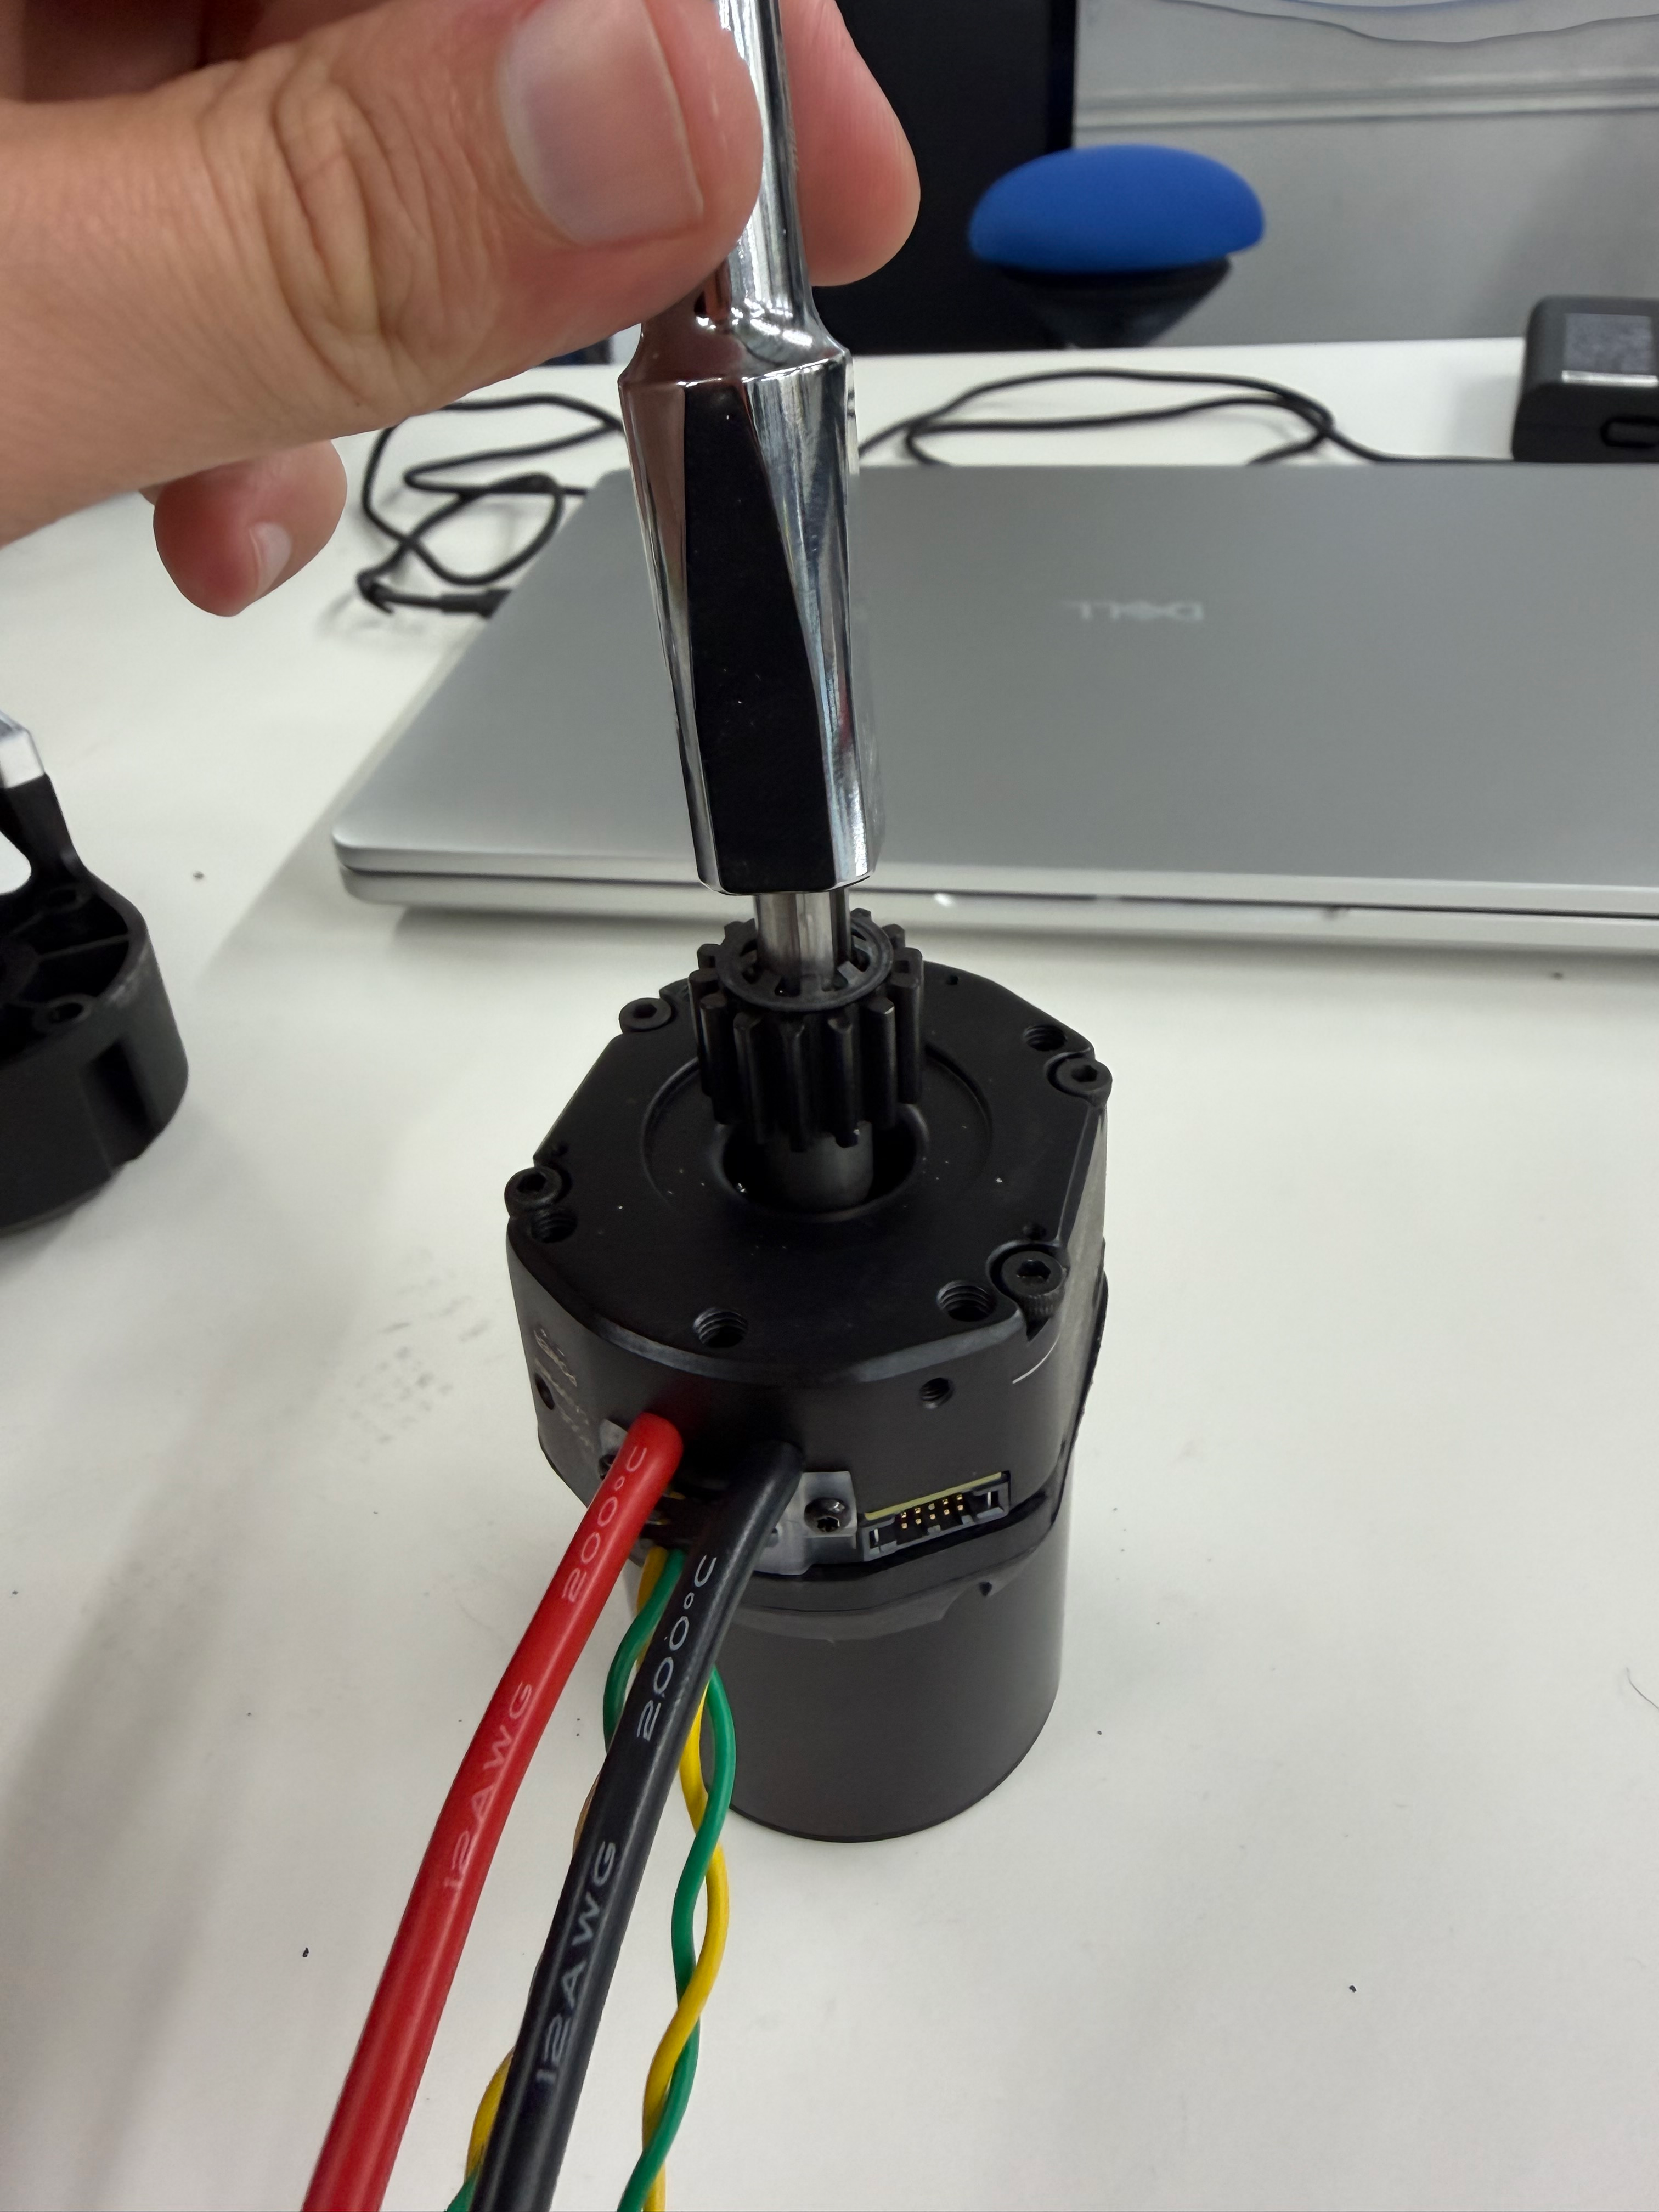
\includegraphics[width=0.31\textwidth]{media/image15.png}
\caption{Installing the pinion gear and seating the retaining ring with a
socket and rubber mallet.}
\end{figure}

\clearpage
Insert the motor assembly in the steering motor slot (side opposite of
the metal gear-ratio plate) through the bottom of the swerve module. Be
sure to leave all cables, ports, and buttons facing outwards and are
accessible. Align three of the mounting holes on the motor controller
with the three mounting points on the module. Use three of the six
provided 10-32 x 1/2'' socket screws to secure the motor assembly.

\begin{warningbox}
Careful not to over-tighten the motor assembly screws.
\end{warningbox}

\begin{figure}[H]
\centering
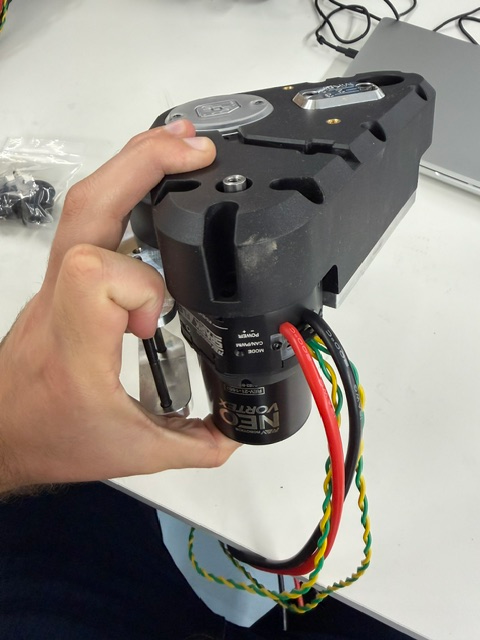
\includegraphics[width=0.5\textwidth]{media/image16.png}
\caption{The steer motor secured in the module slot opposite the
gear-ratio plate.}
\end{figure}

\clearpage
\assemblystep{Drive Motor Installation}
The second motor will require the R1 drive pinion gear, 2mm machine key,
and the provided 10-32 x 3/8'' button screw (T25 head).

\begin{figure}[H]
\centering
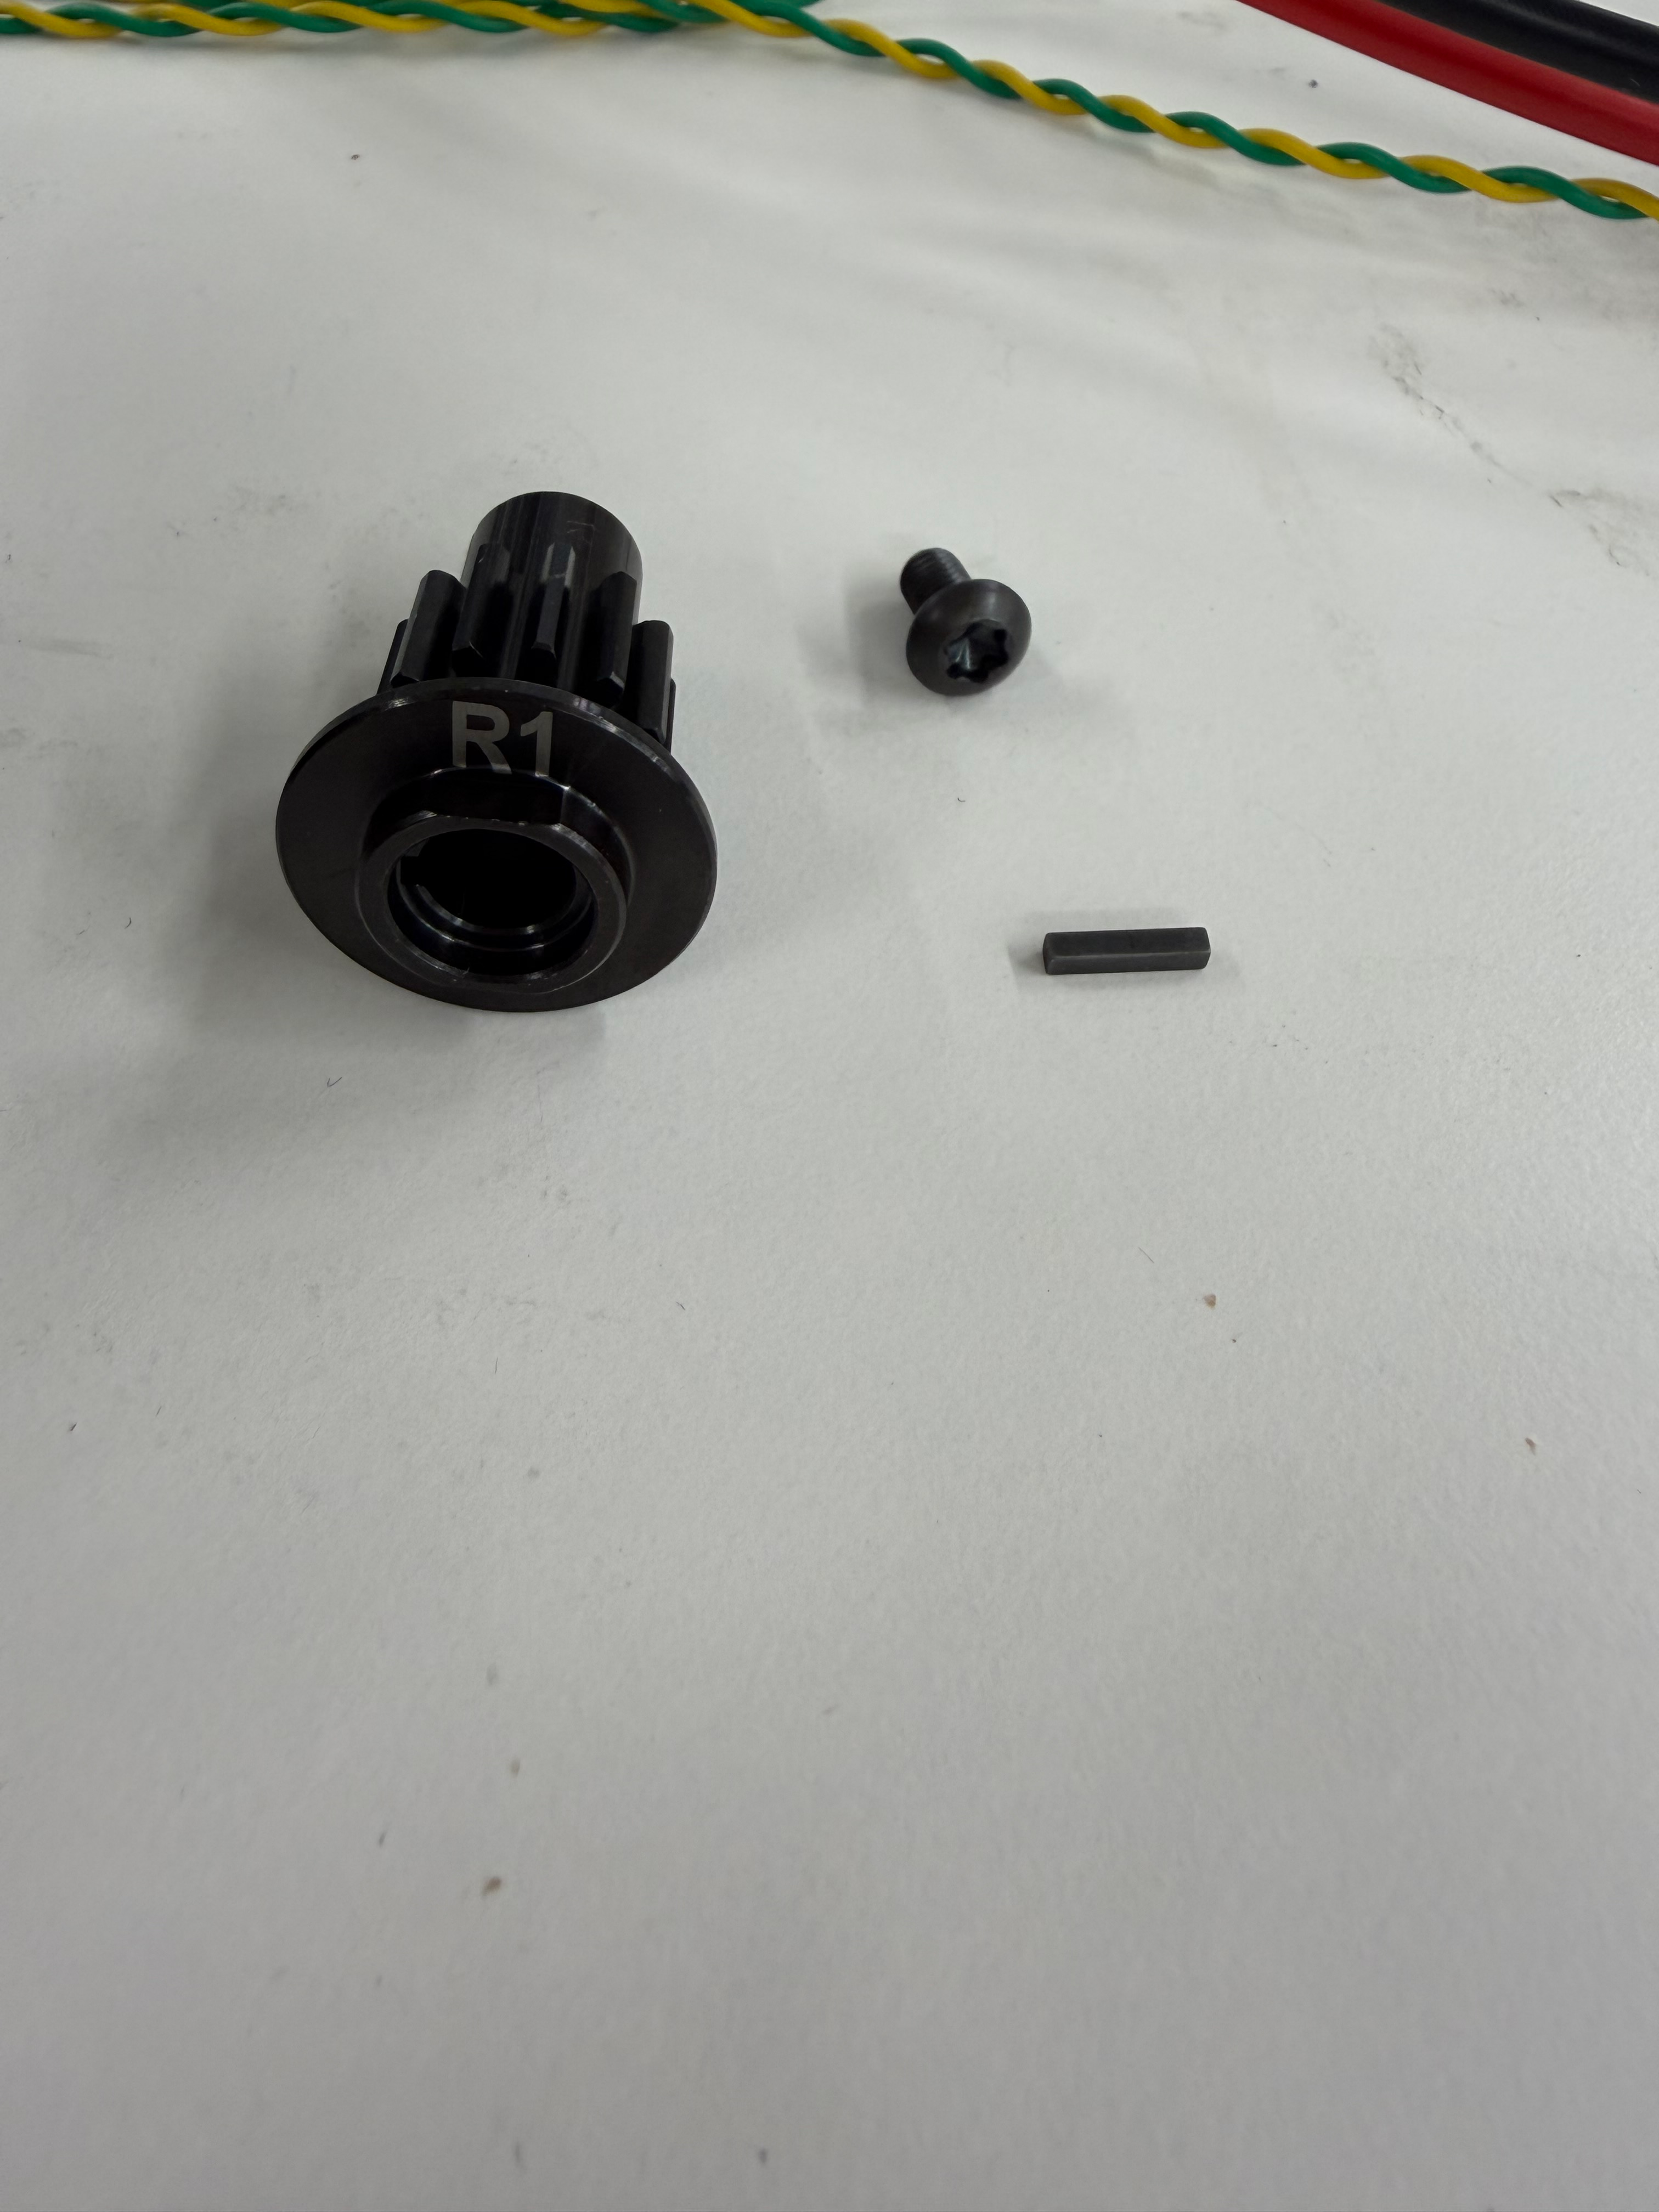
\includegraphics[width=0.5\textwidth]{media/image17.png}
\caption{Drive motor hardware: R1 drive pinion gear, machine key, and
button head screw.}
\end{figure}

Install the machine key into the motor shaft. Insert the motor assembly
into the drive motor slot (side with the metal gear-ratio plate) through
the bottom of the swerve module. Keep motor either perpendicular or if
tilted, leave the shaft slot facing upwards as the machine key may fall
out. Be sure to leave all cables, ports, and buttons facing outwards and
are accessible. Align three of the mounting holes on the motor
controller with the three mounting points on the module. Use three of
the six provided 10-32 x 1/2'' socket screws to secure the motor
assembly. Insert the drive pinion gear, making sure to align the slot
with the machine key. Tighten with the button head screw.

\begin{warningbox}
Careful not to over-tighten the motor assembly screws.
\end{warningbox}

\begin{figure}[H]
\centering
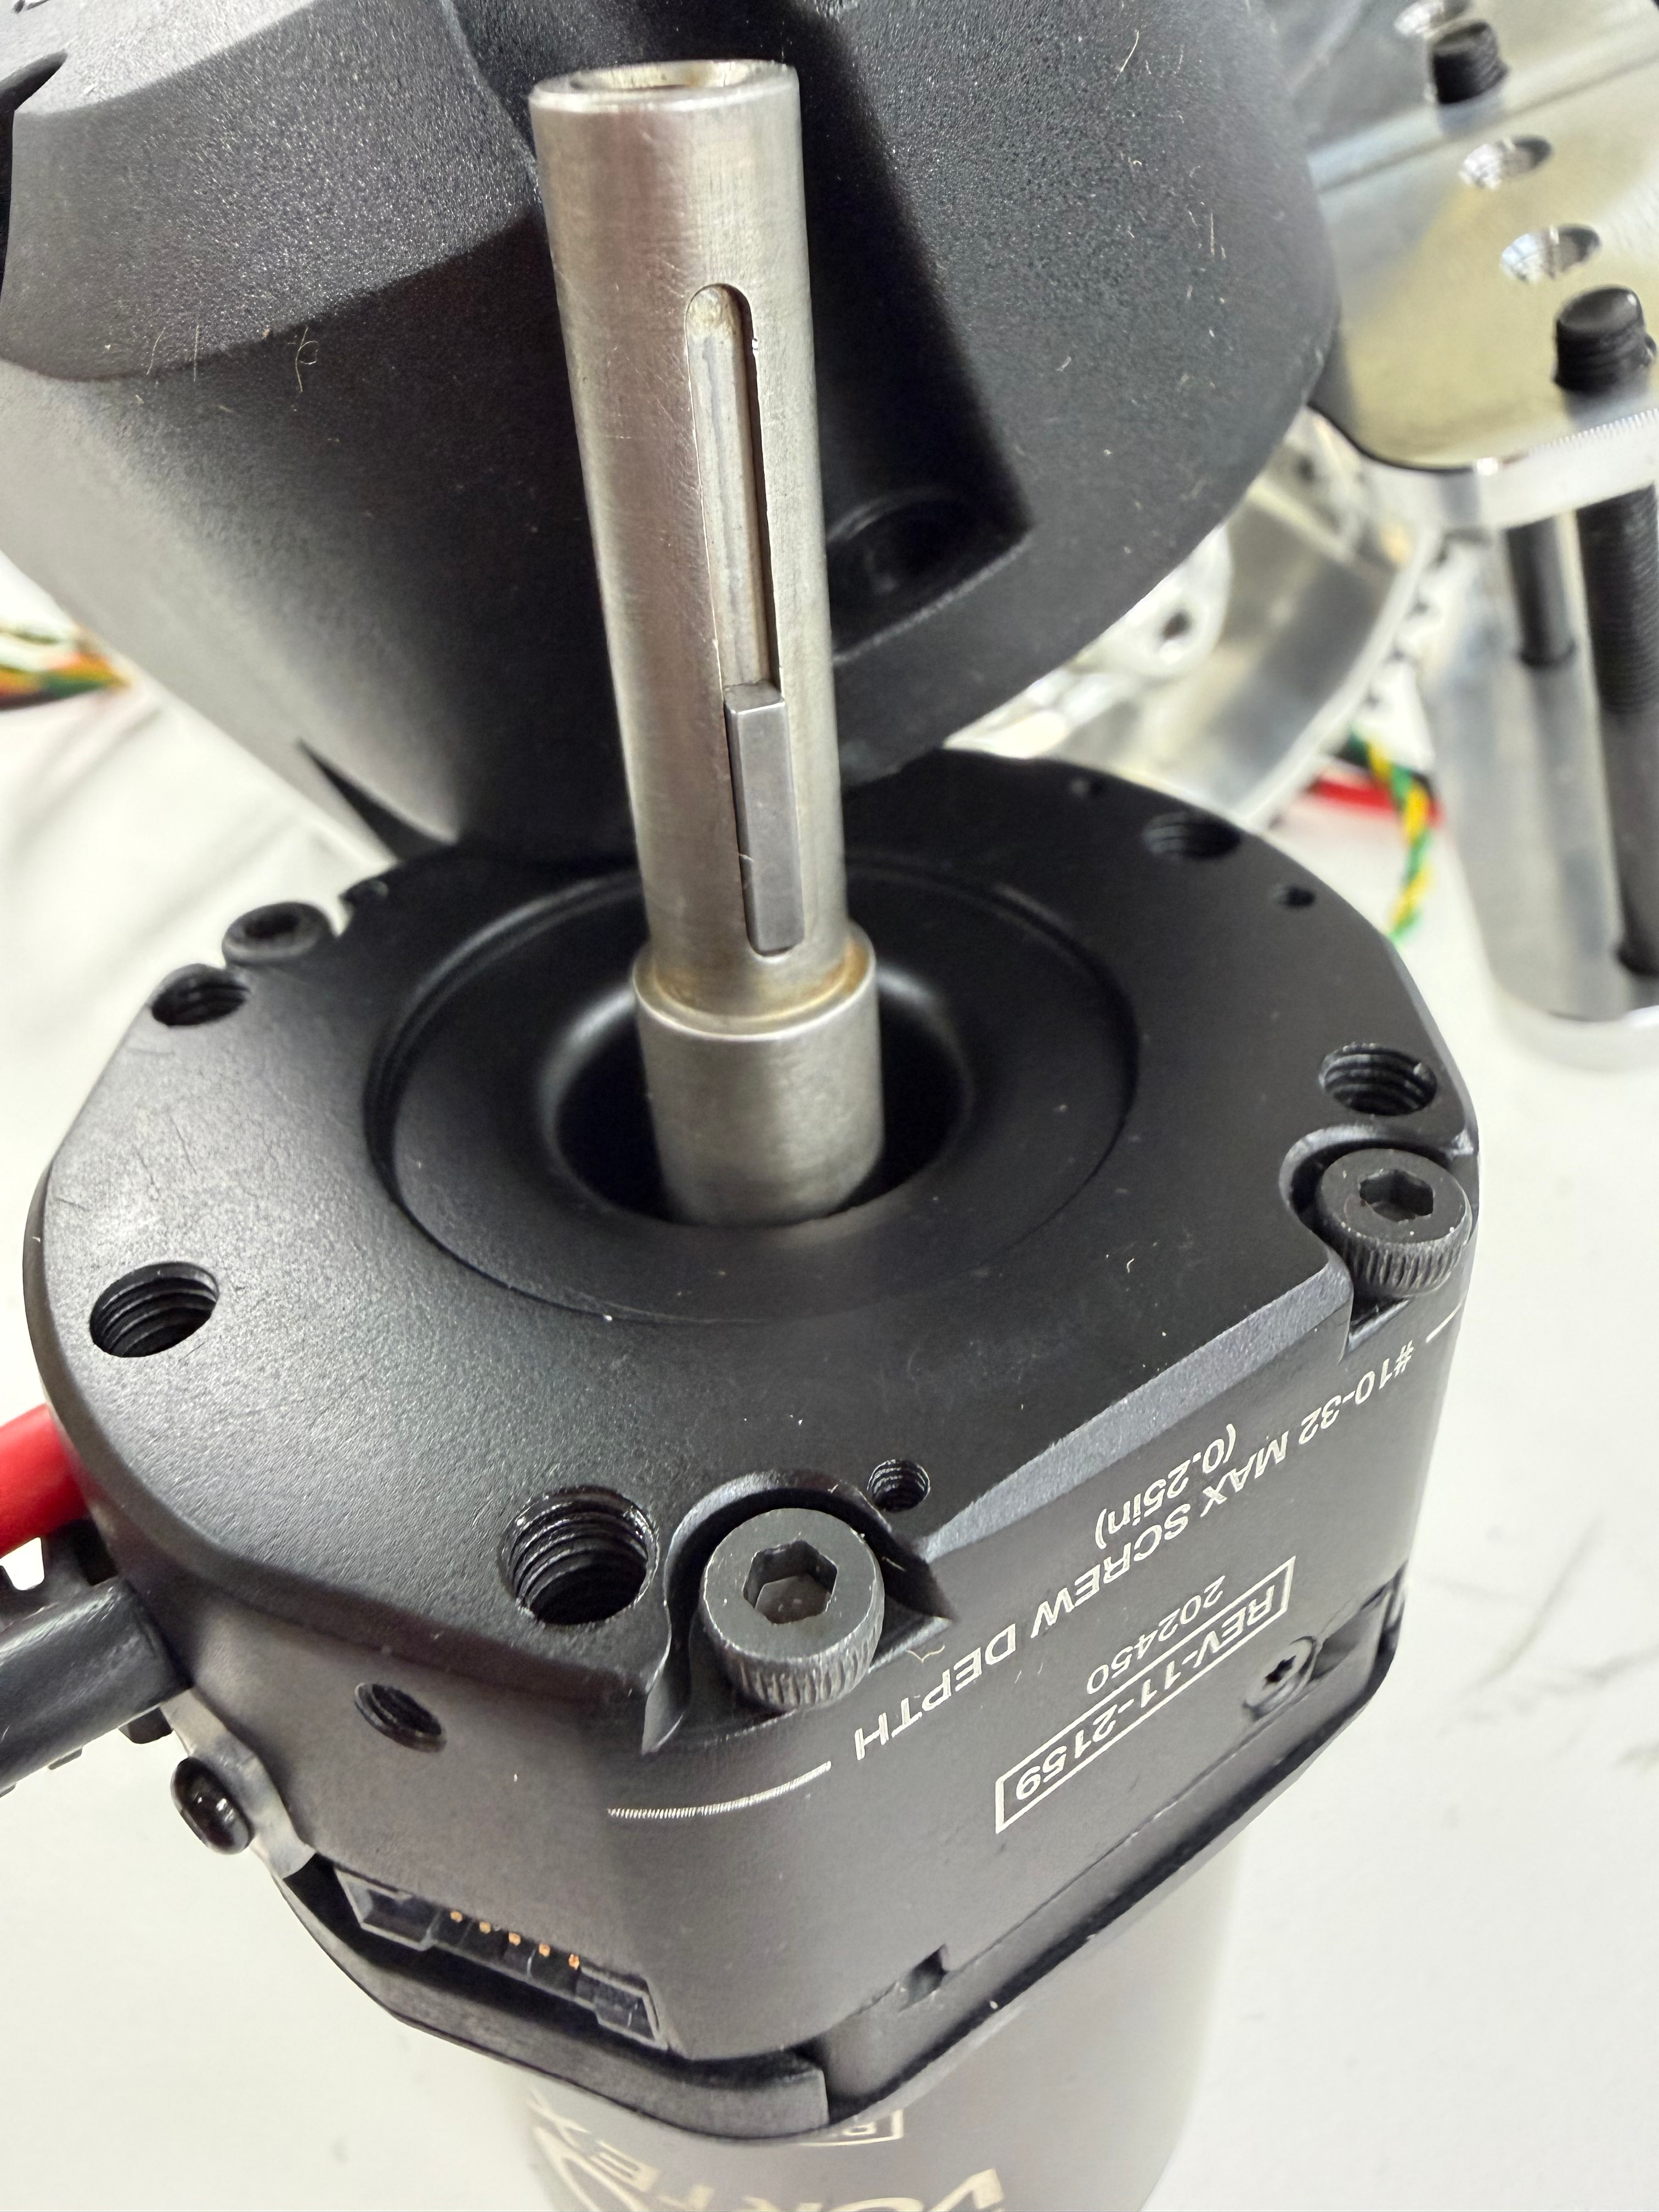
\includegraphics[width=0.47\textwidth]{media/image18.png}
\hfill
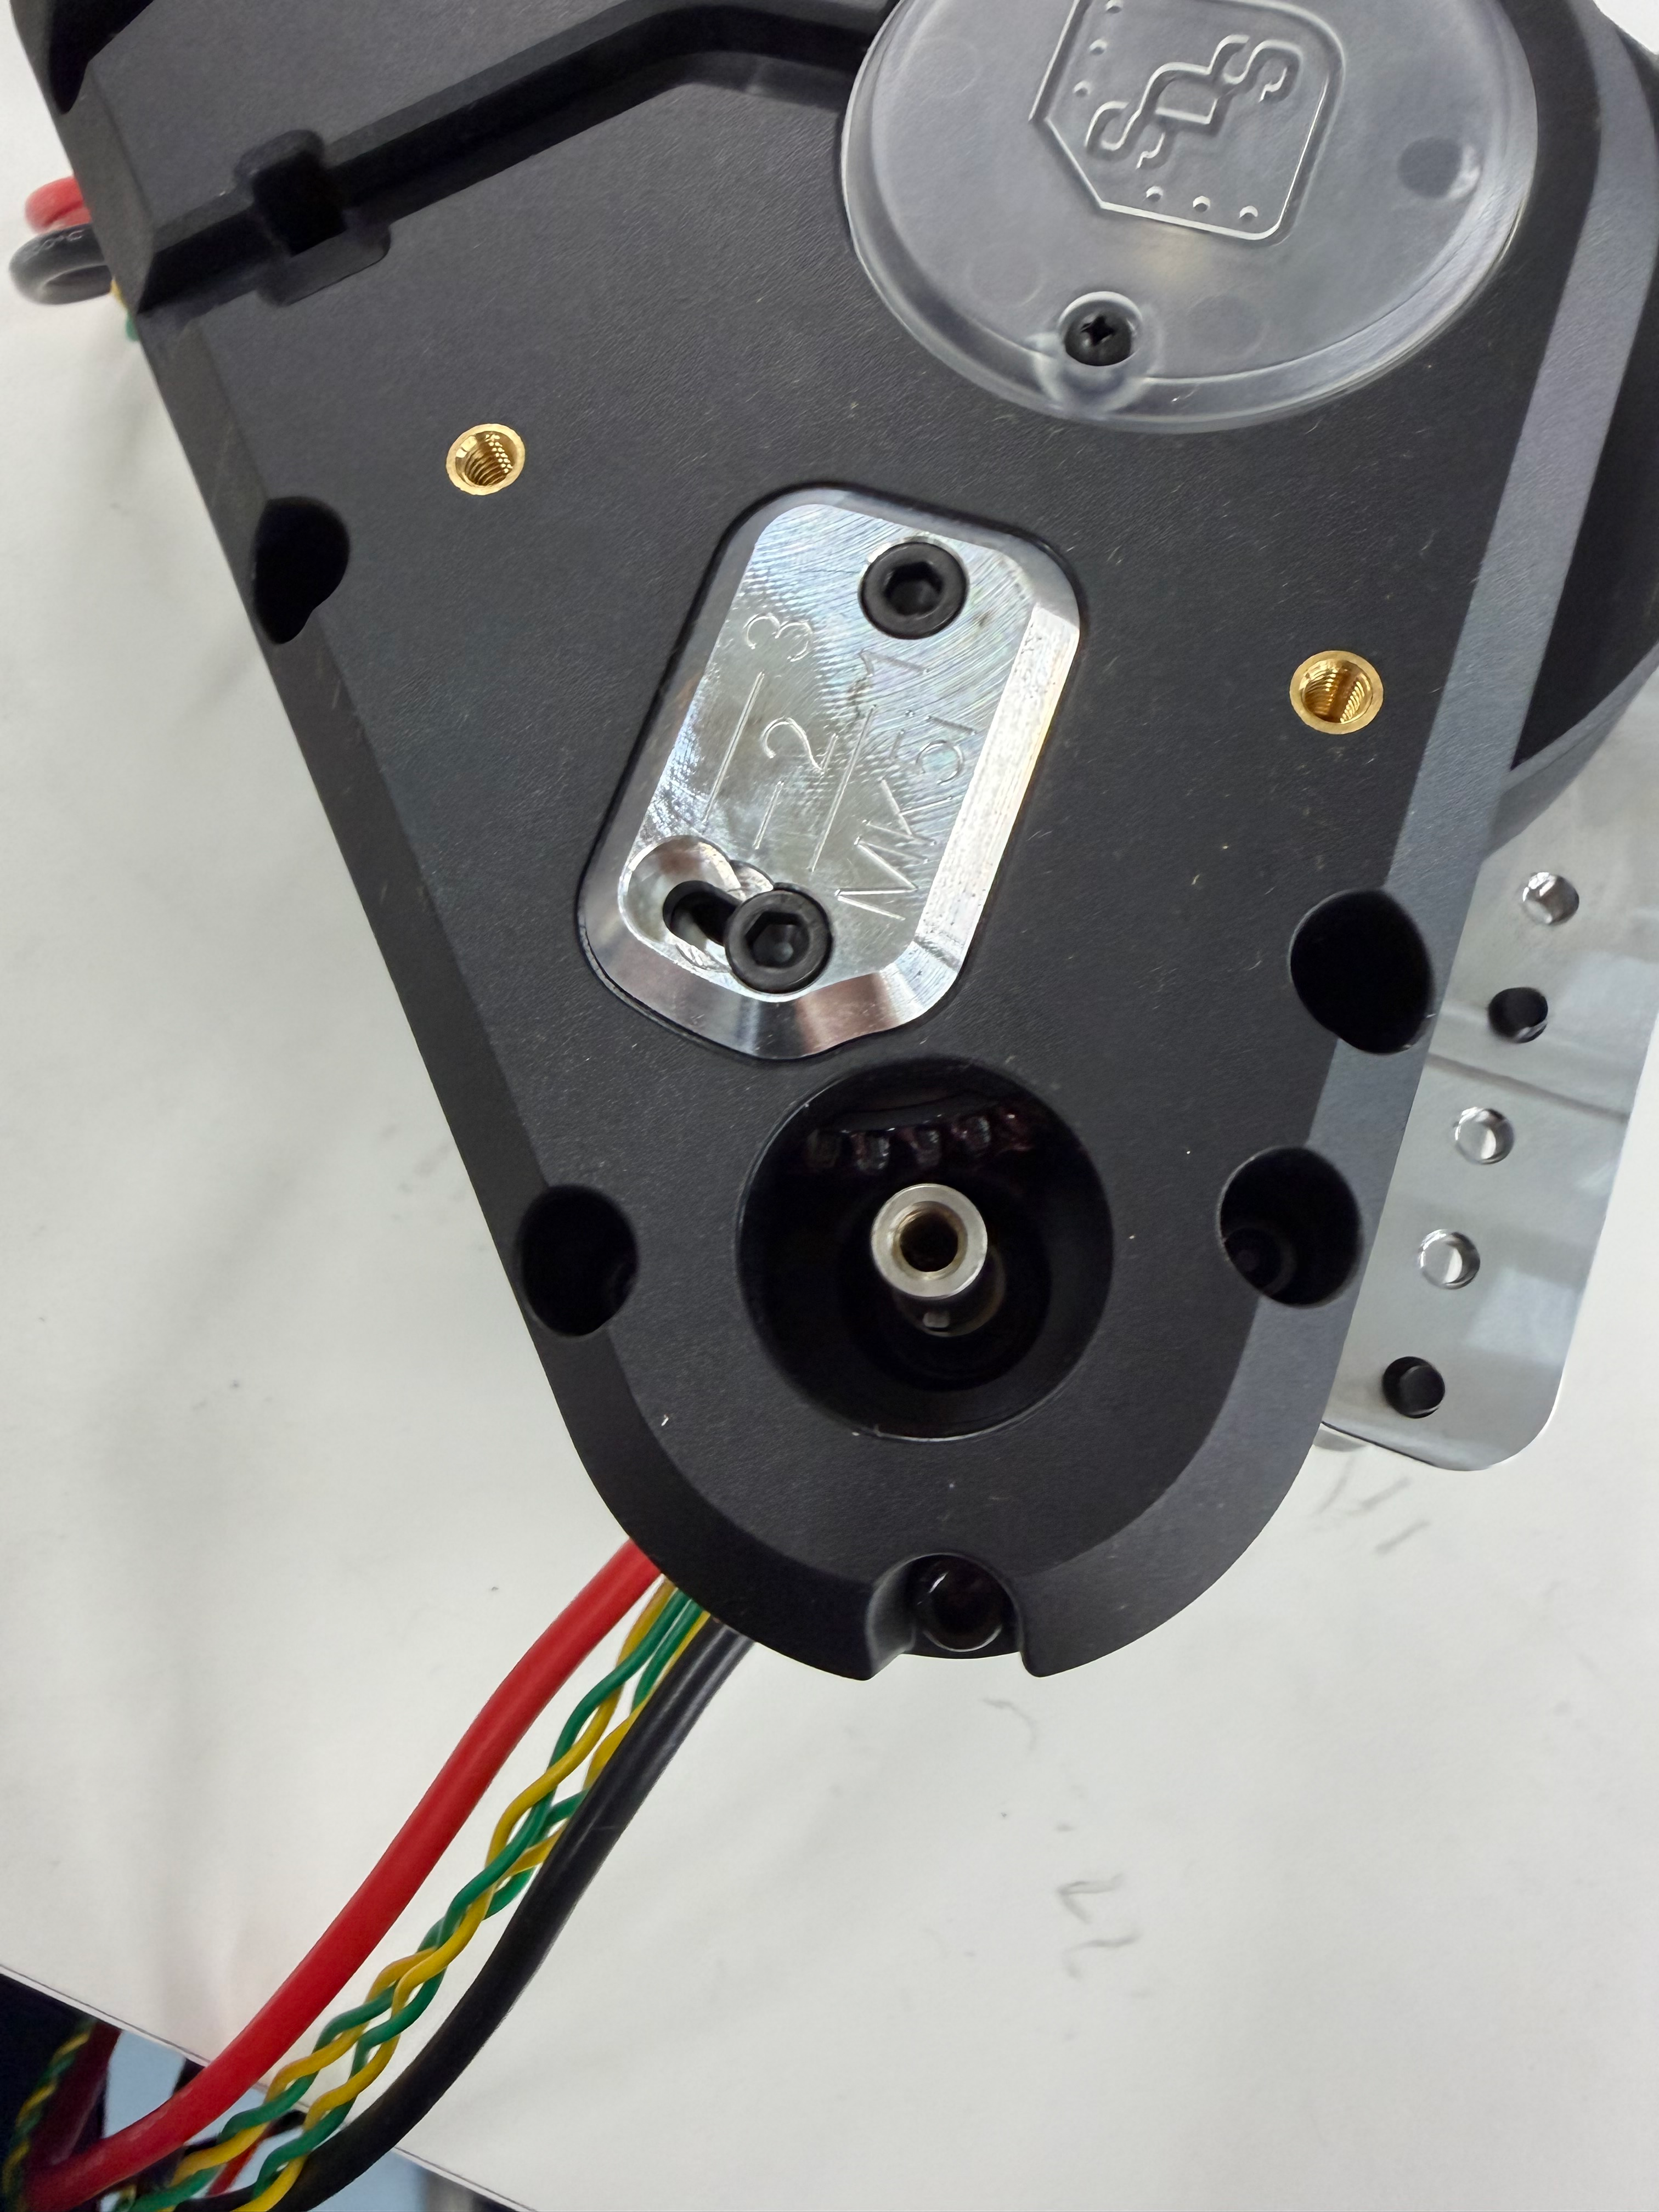
\includegraphics[width=0.47\textwidth]{media/image19.png}

\vspace{0.4cm}
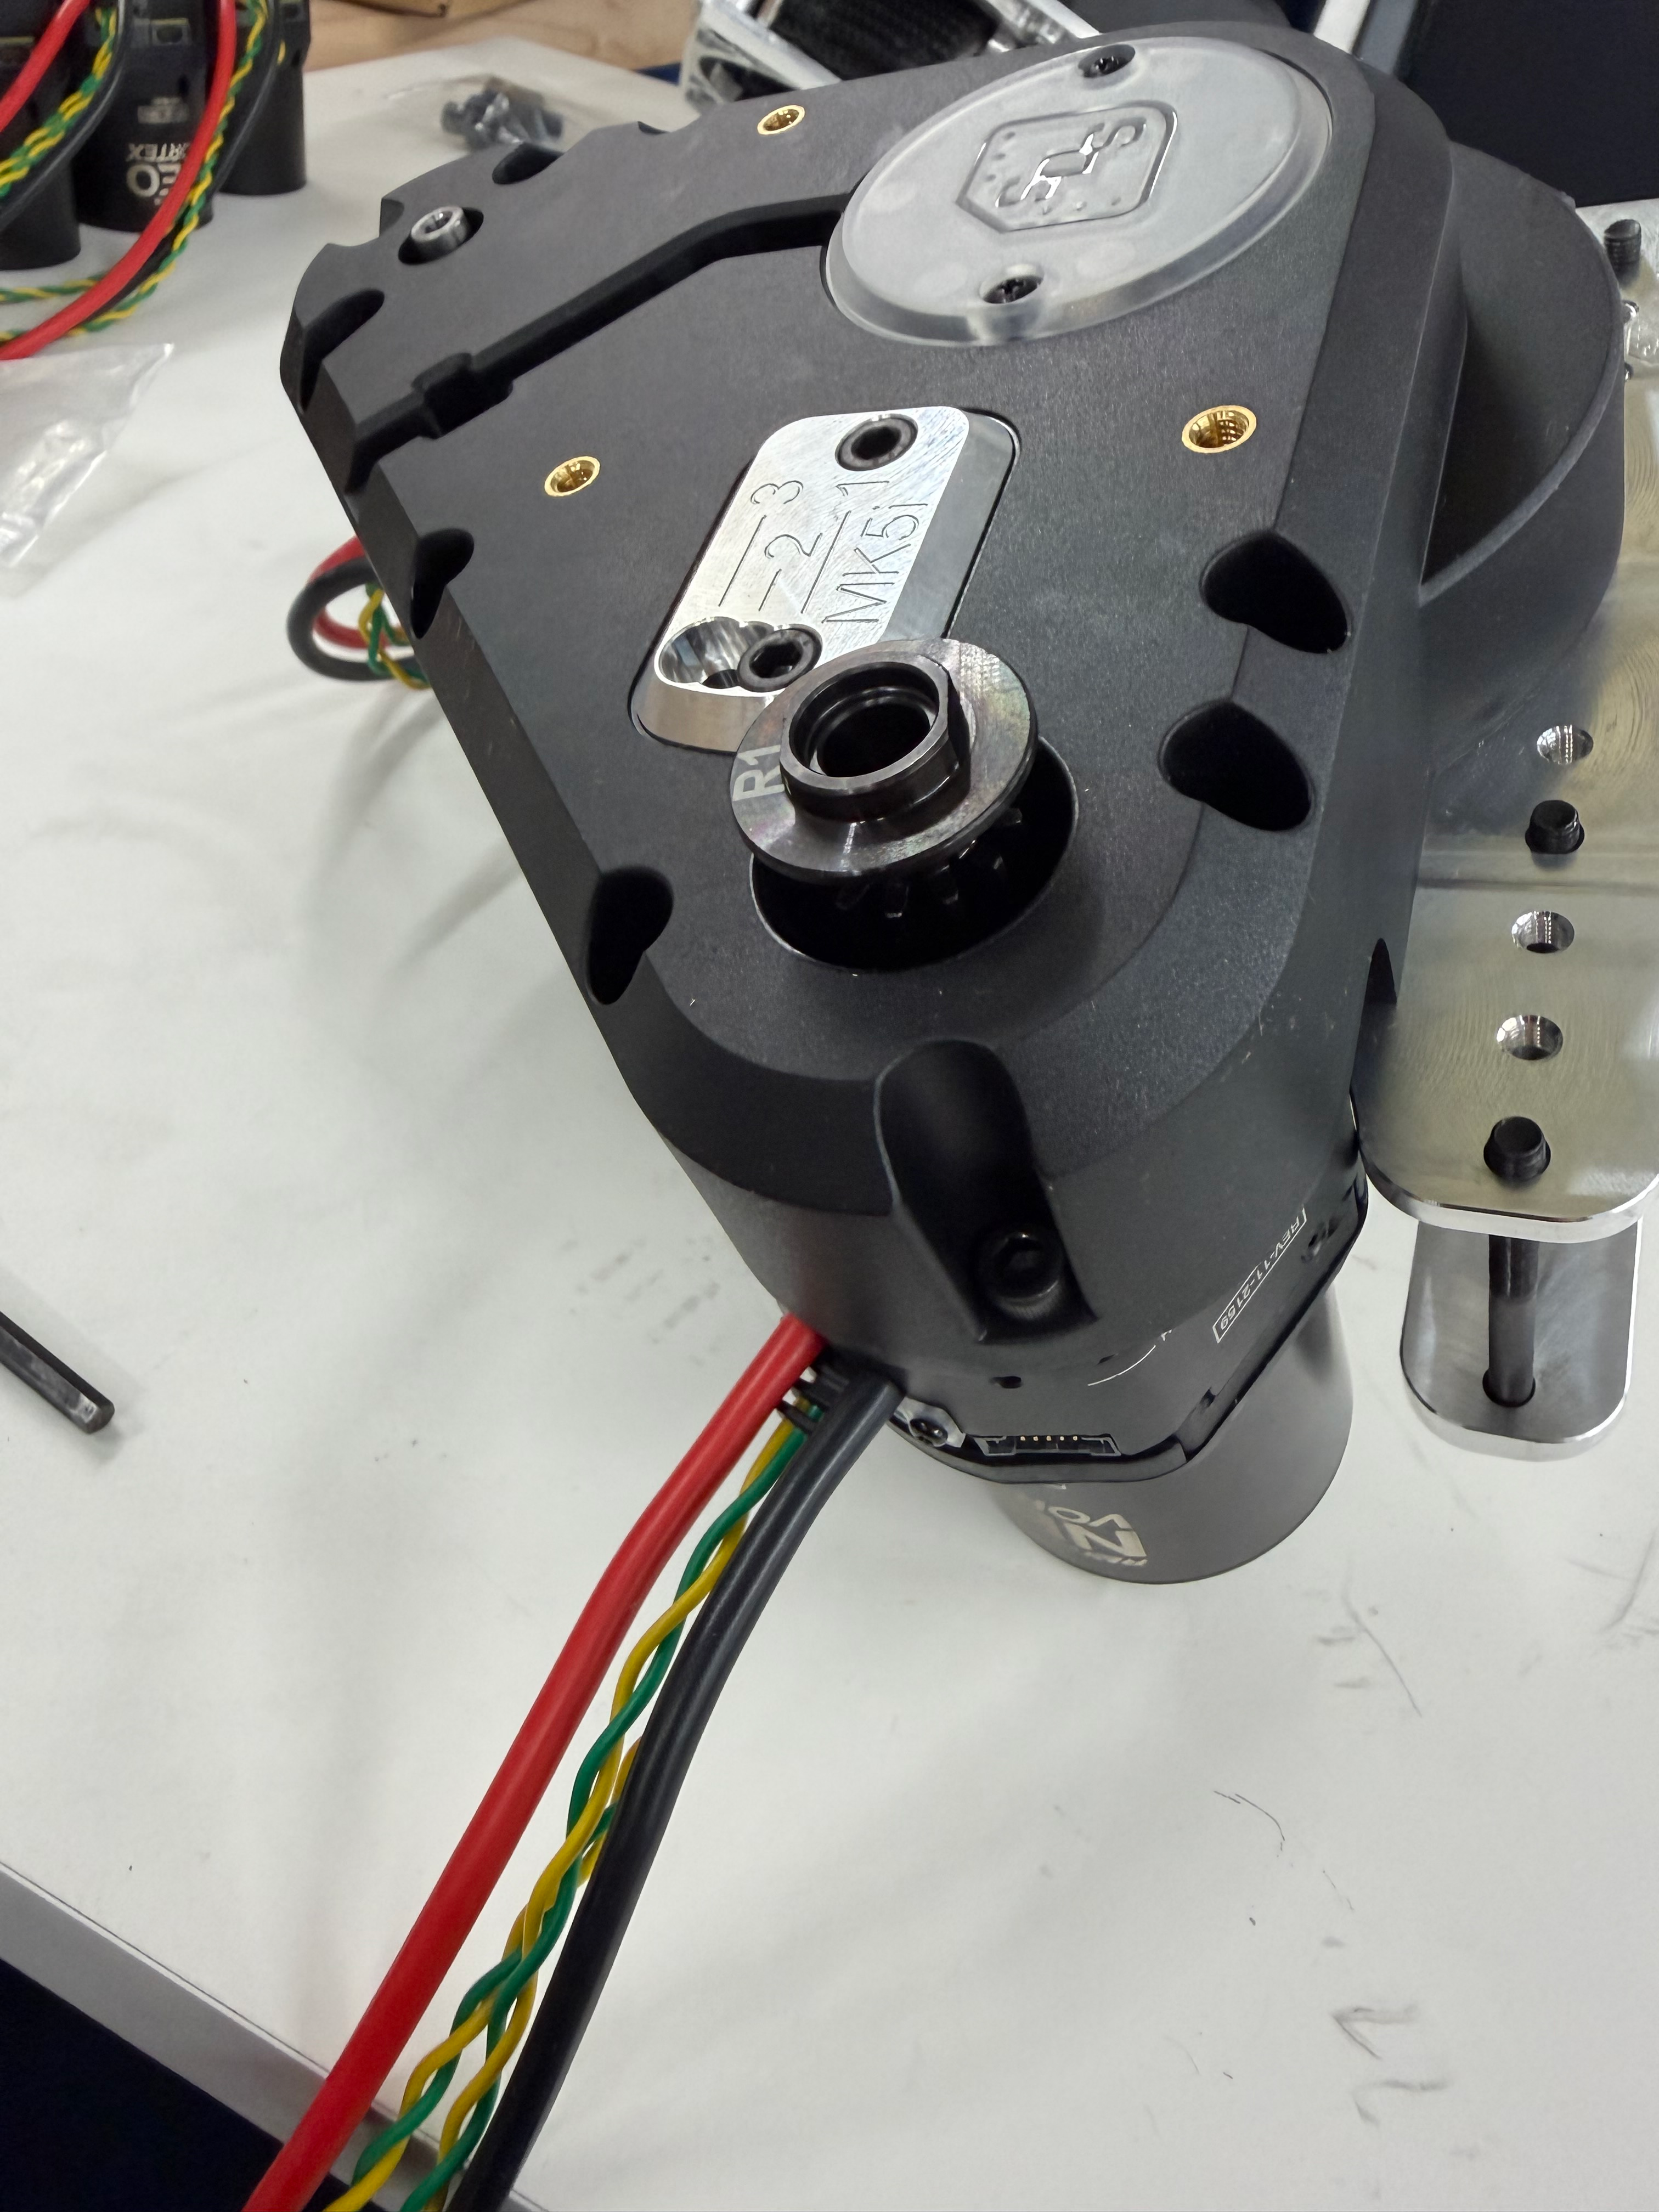
\includegraphics[width=0.47\textwidth]{media/image20.png}
\hfill
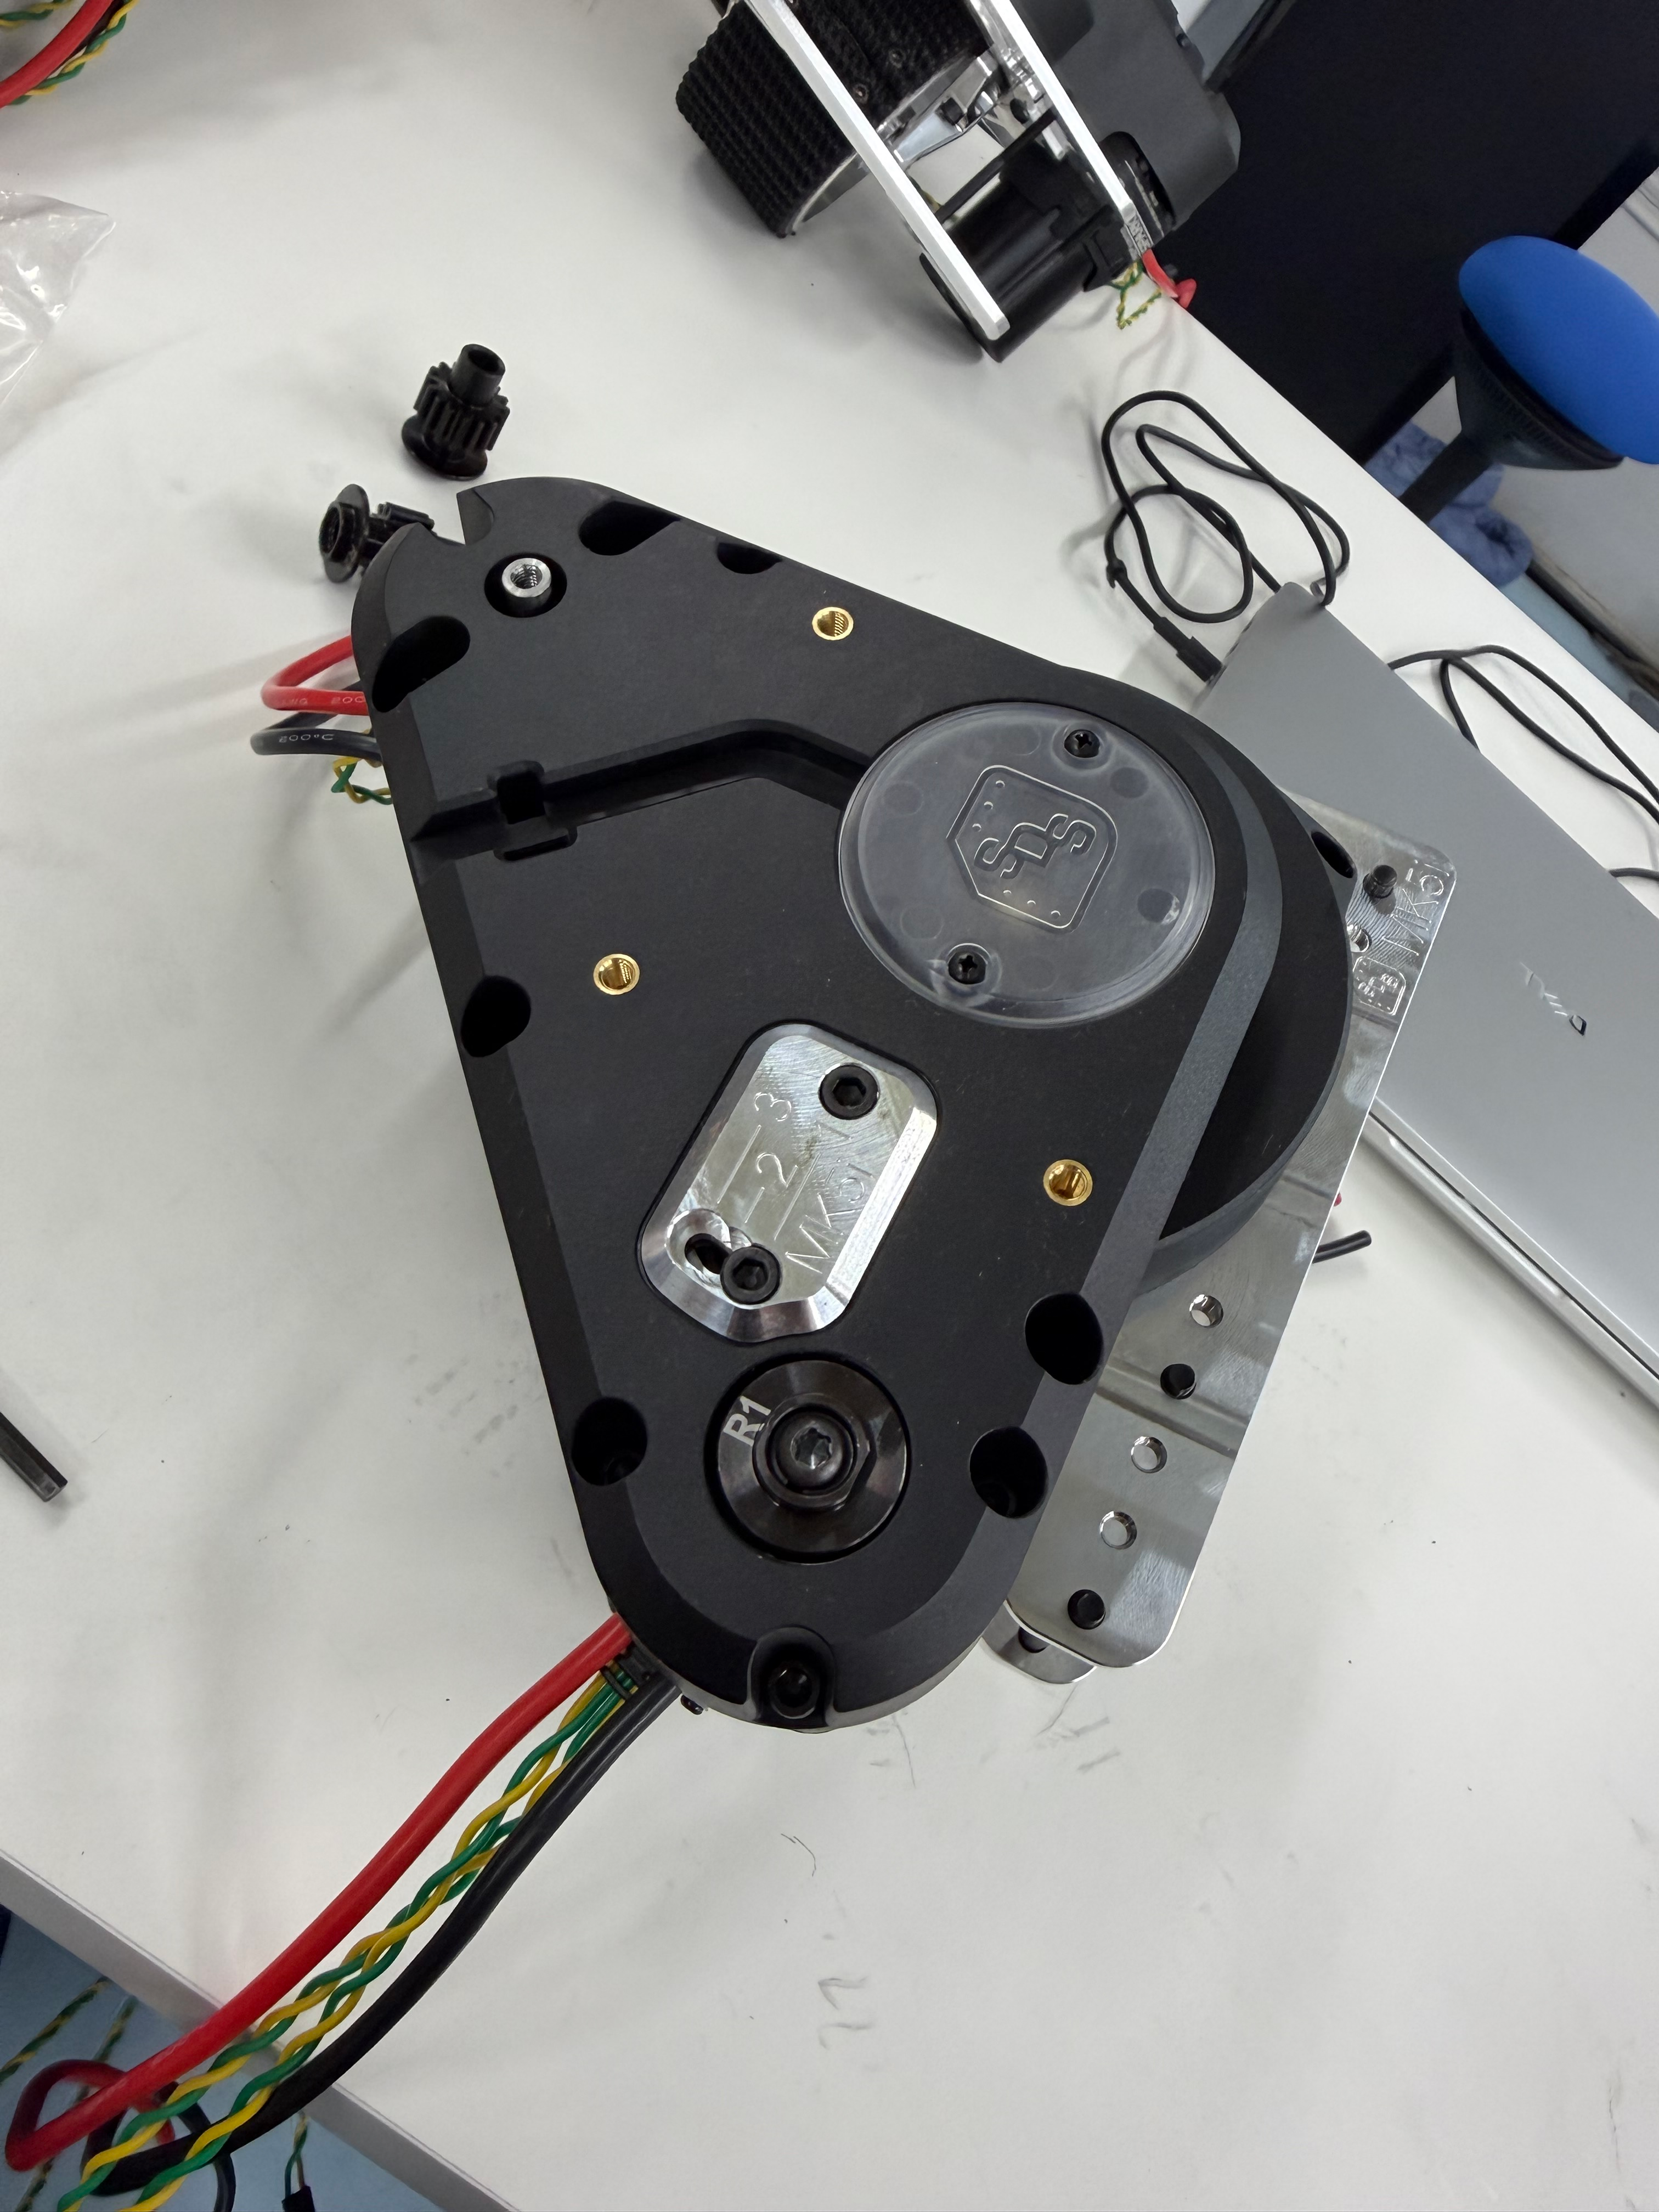
\includegraphics[width=0.47\textwidth]{media/image21.png}
\caption{Mounting the drive motor and seating the drive pinion gear on
the keyed shaft.}
\end{figure}

\assemblystep{Encoder Installation}

\begin{figure}[H]
\centering
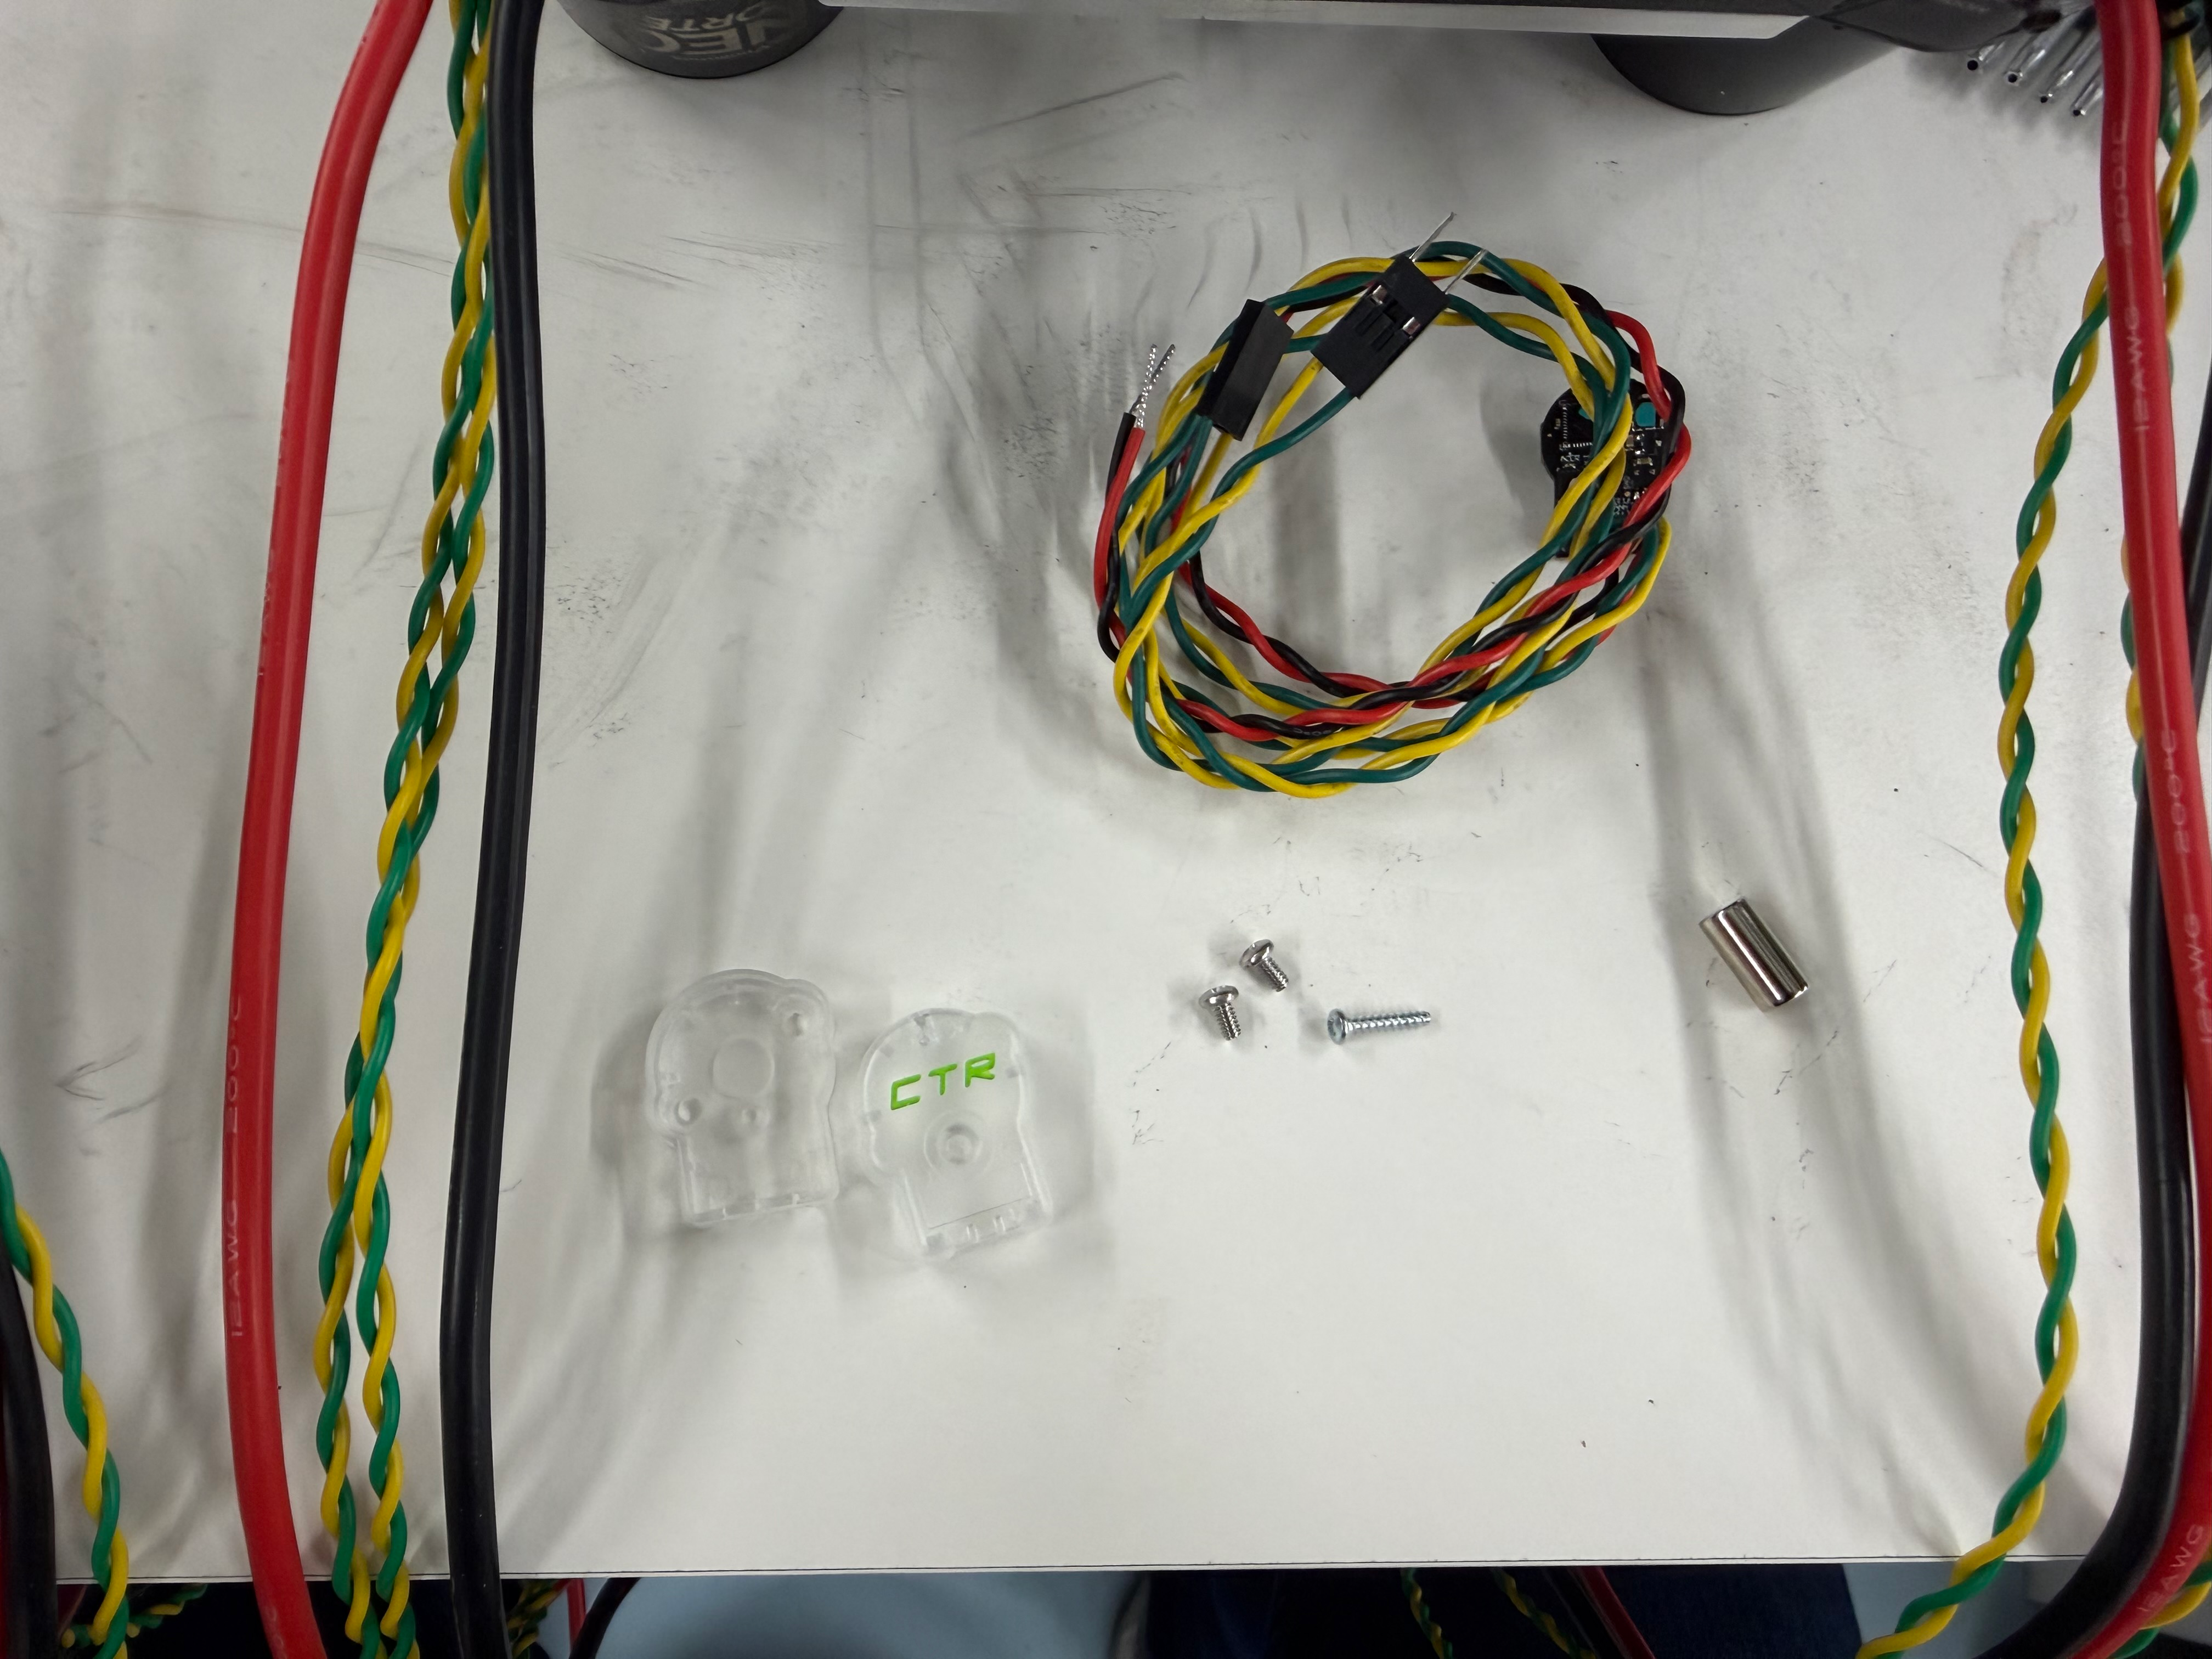
\includegraphics[width=0.5\textwidth]{media/image22.png}
\caption{The CANcoder encoder and its clear plastic cover.}
\end{figure}

Remove the two 4-20 x 3/8'' thread-forming screws from the clear plastic
encoder cover. If there is no magnet inside the module or if the magnet
is loose, insert the magnet and secure with Loctite. Secure the bottom
cover with the two short screws provided with the encoder. Make sure the
rectangular end is facing the wire channel as shown below. Place the
encoder in the bottom cover, followed by the top cover. Secure the top
cover with the other provided screw. Reattach the clear encoder cover.

\begin{warningbox}
Do not over-tighten any screws in this step.
\end{warningbox}

\begin{figure}[H]
\centering
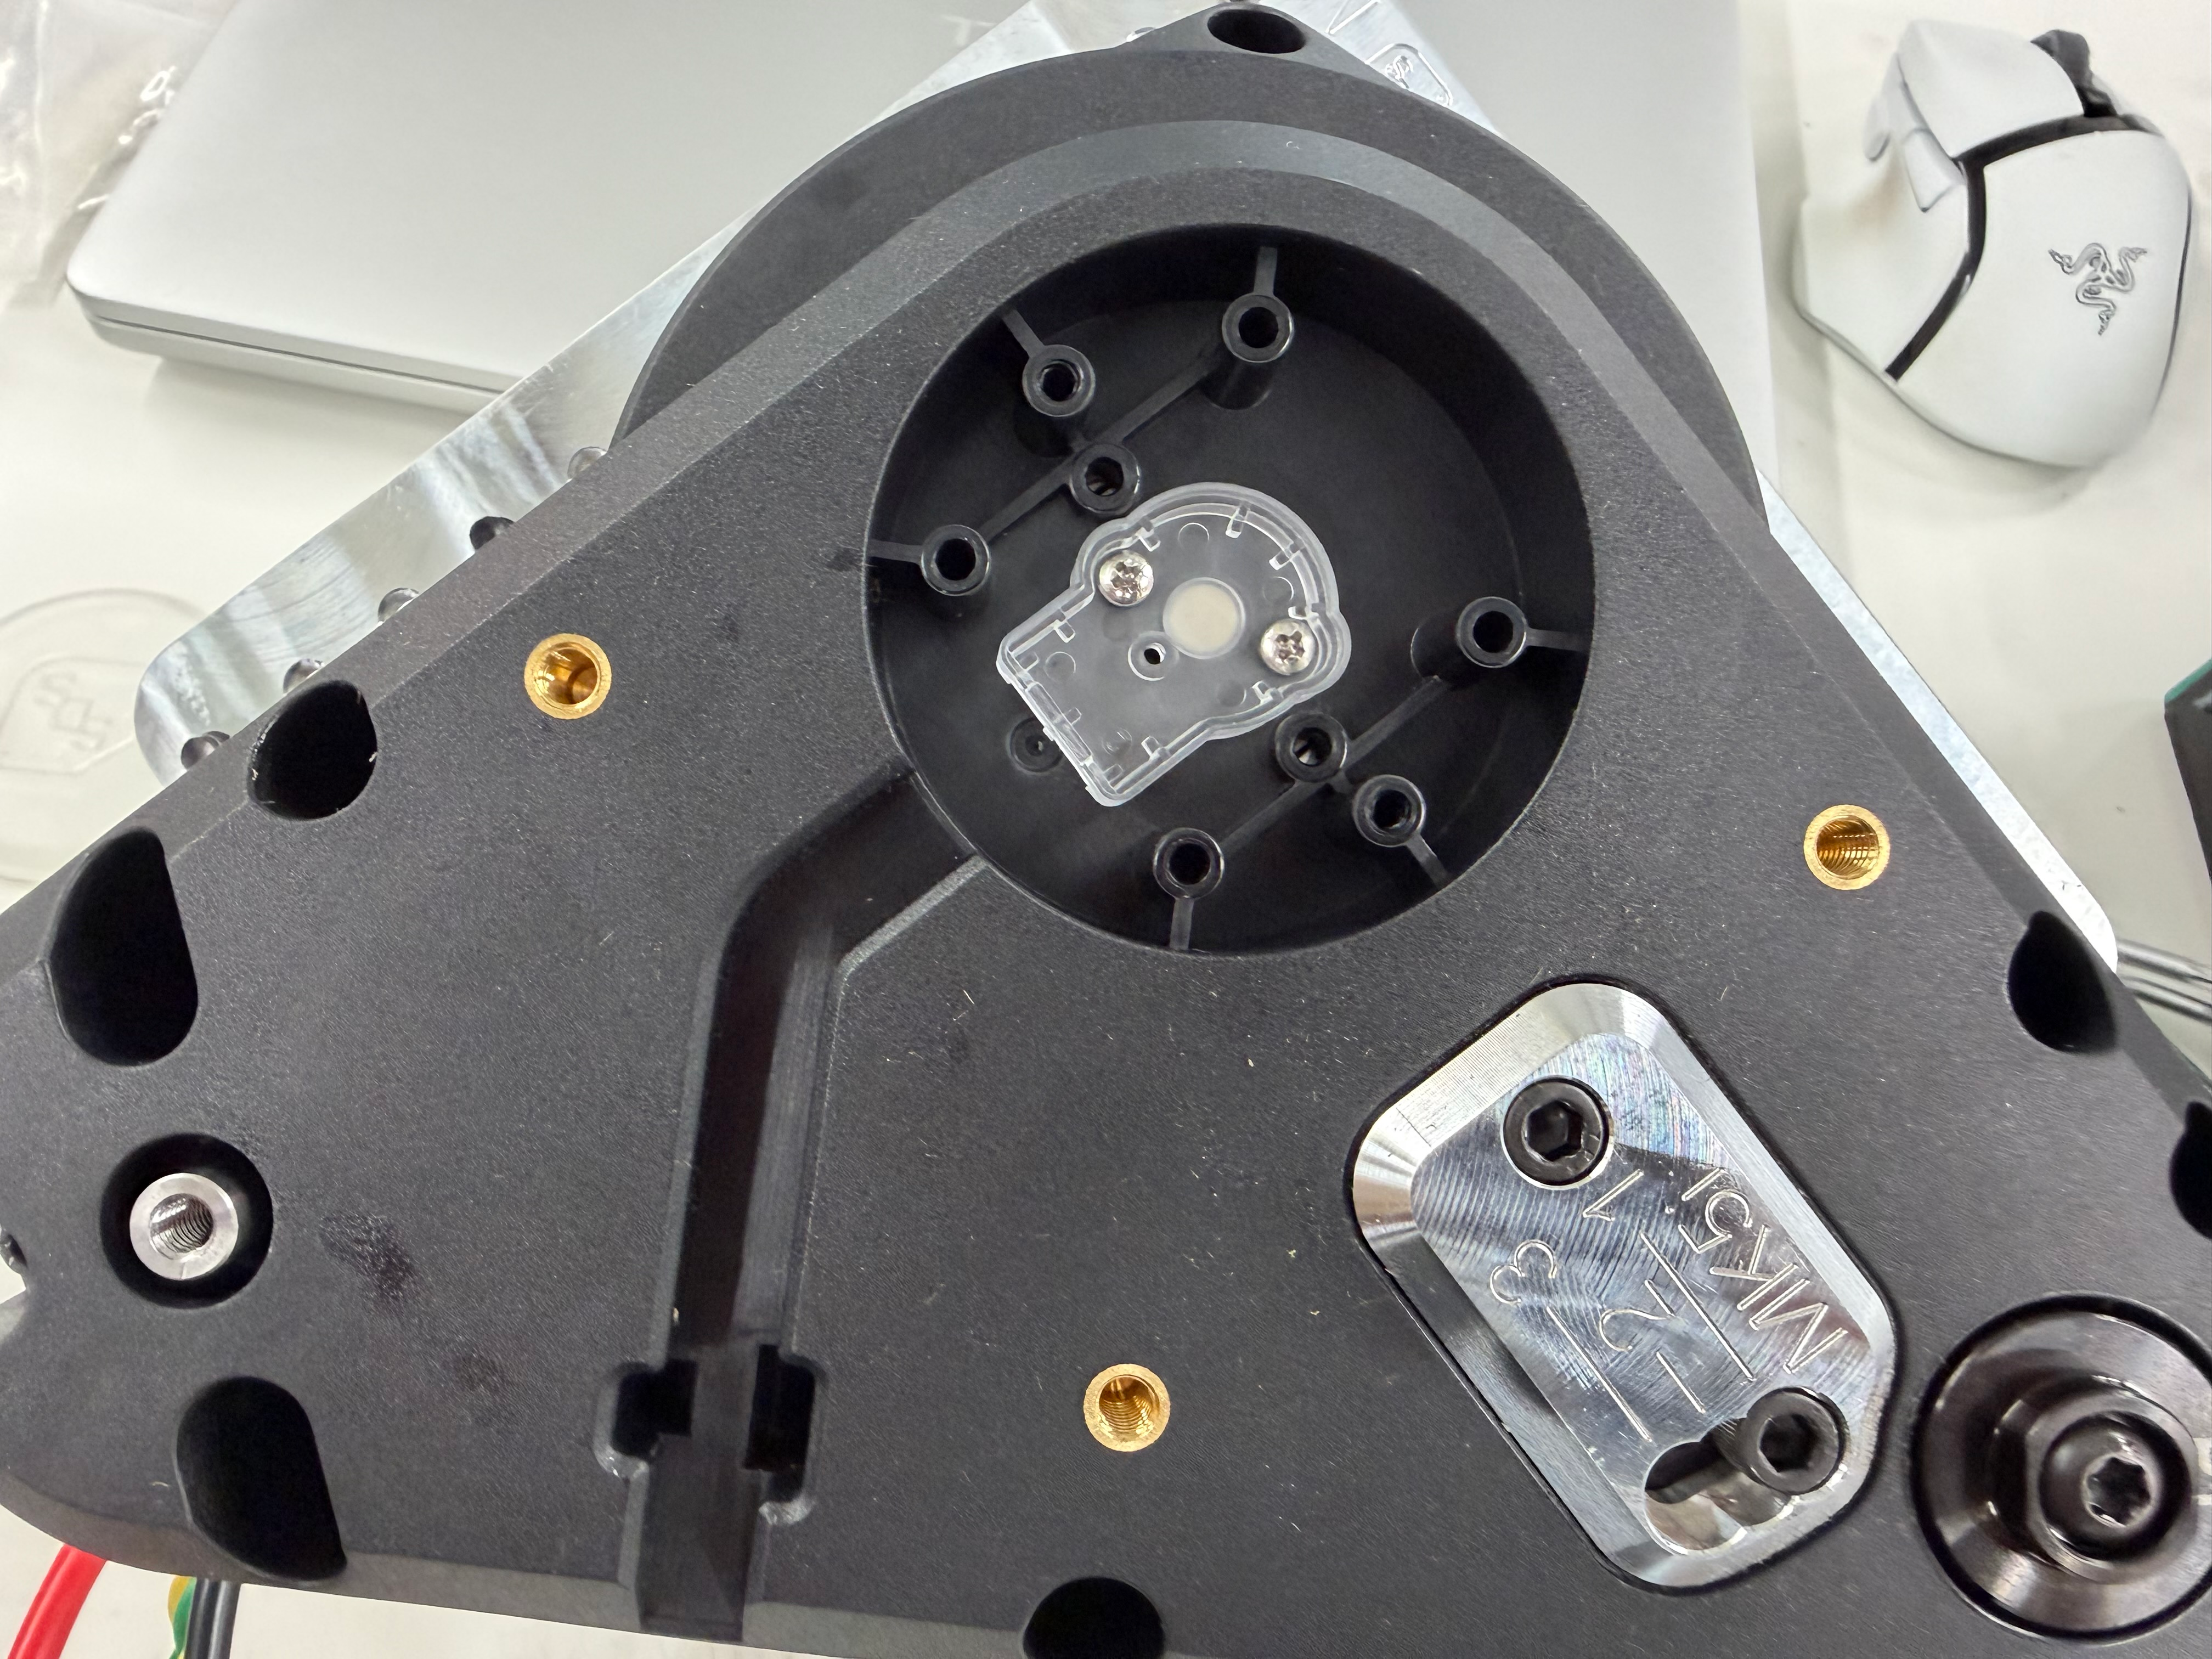
\includegraphics[width=0.31\textwidth]{media/image23.png}
\hfill
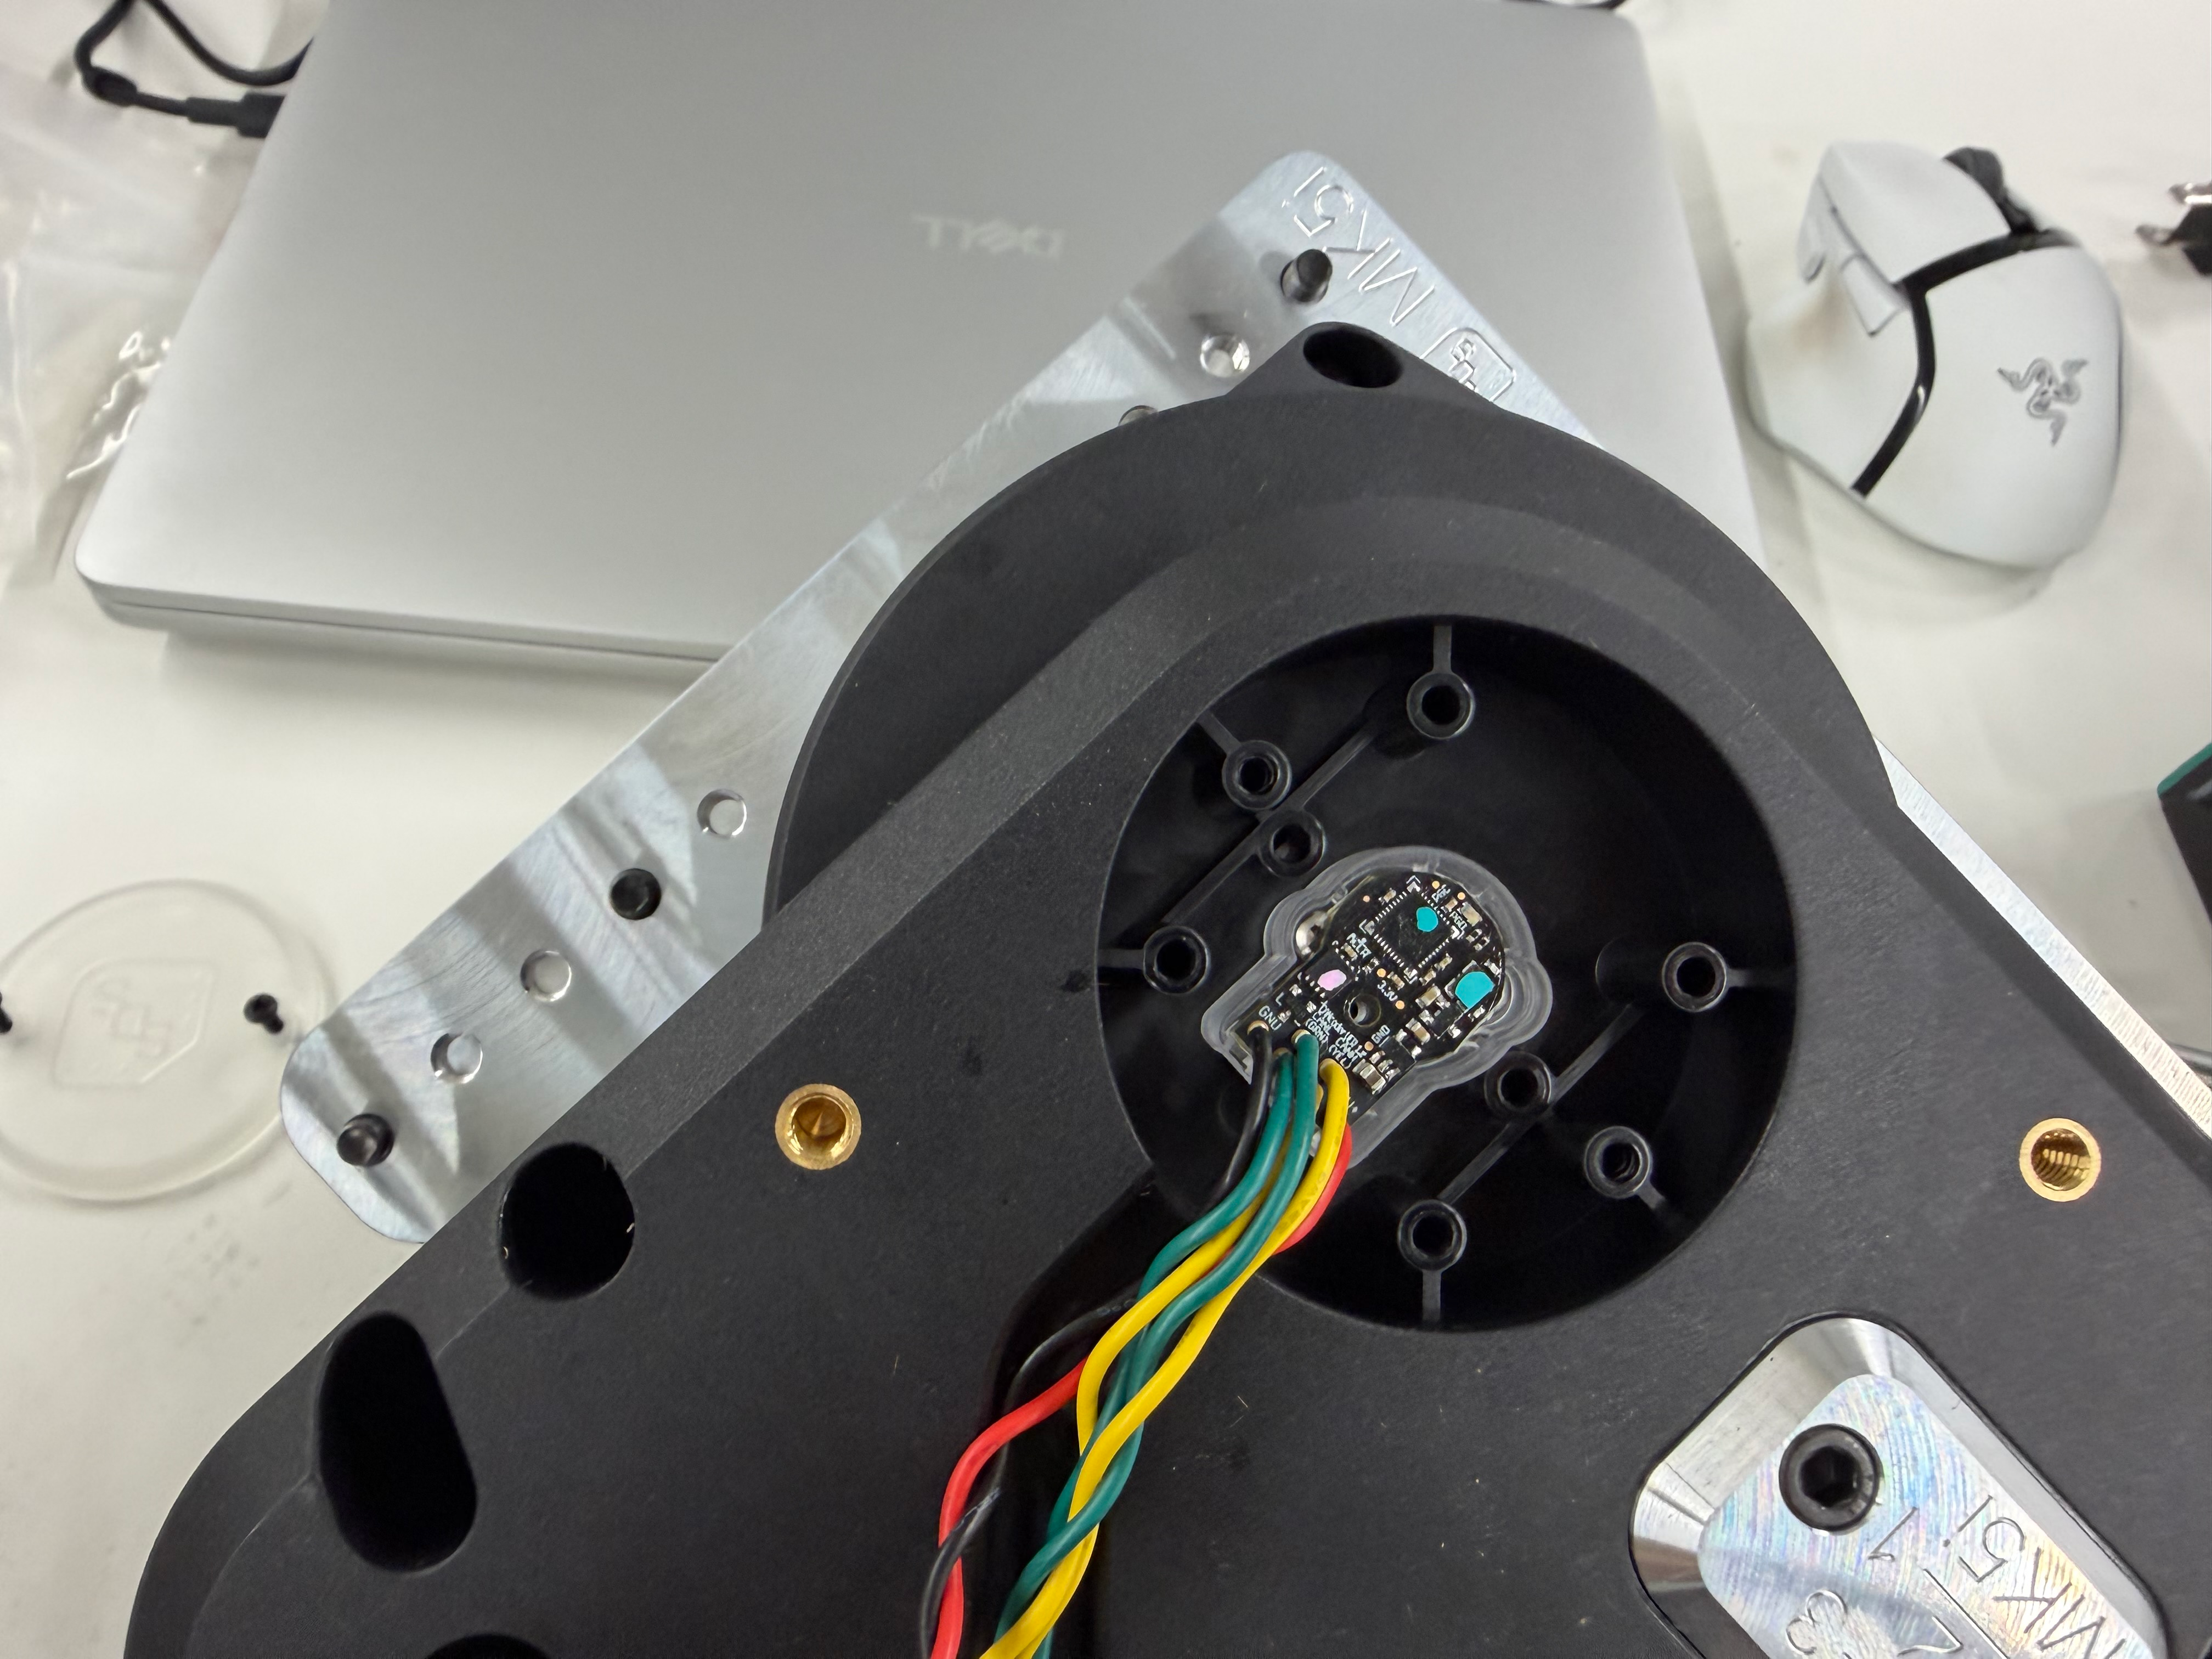
\includegraphics[width=0.31\textwidth]{media/image24.png}
\hfill
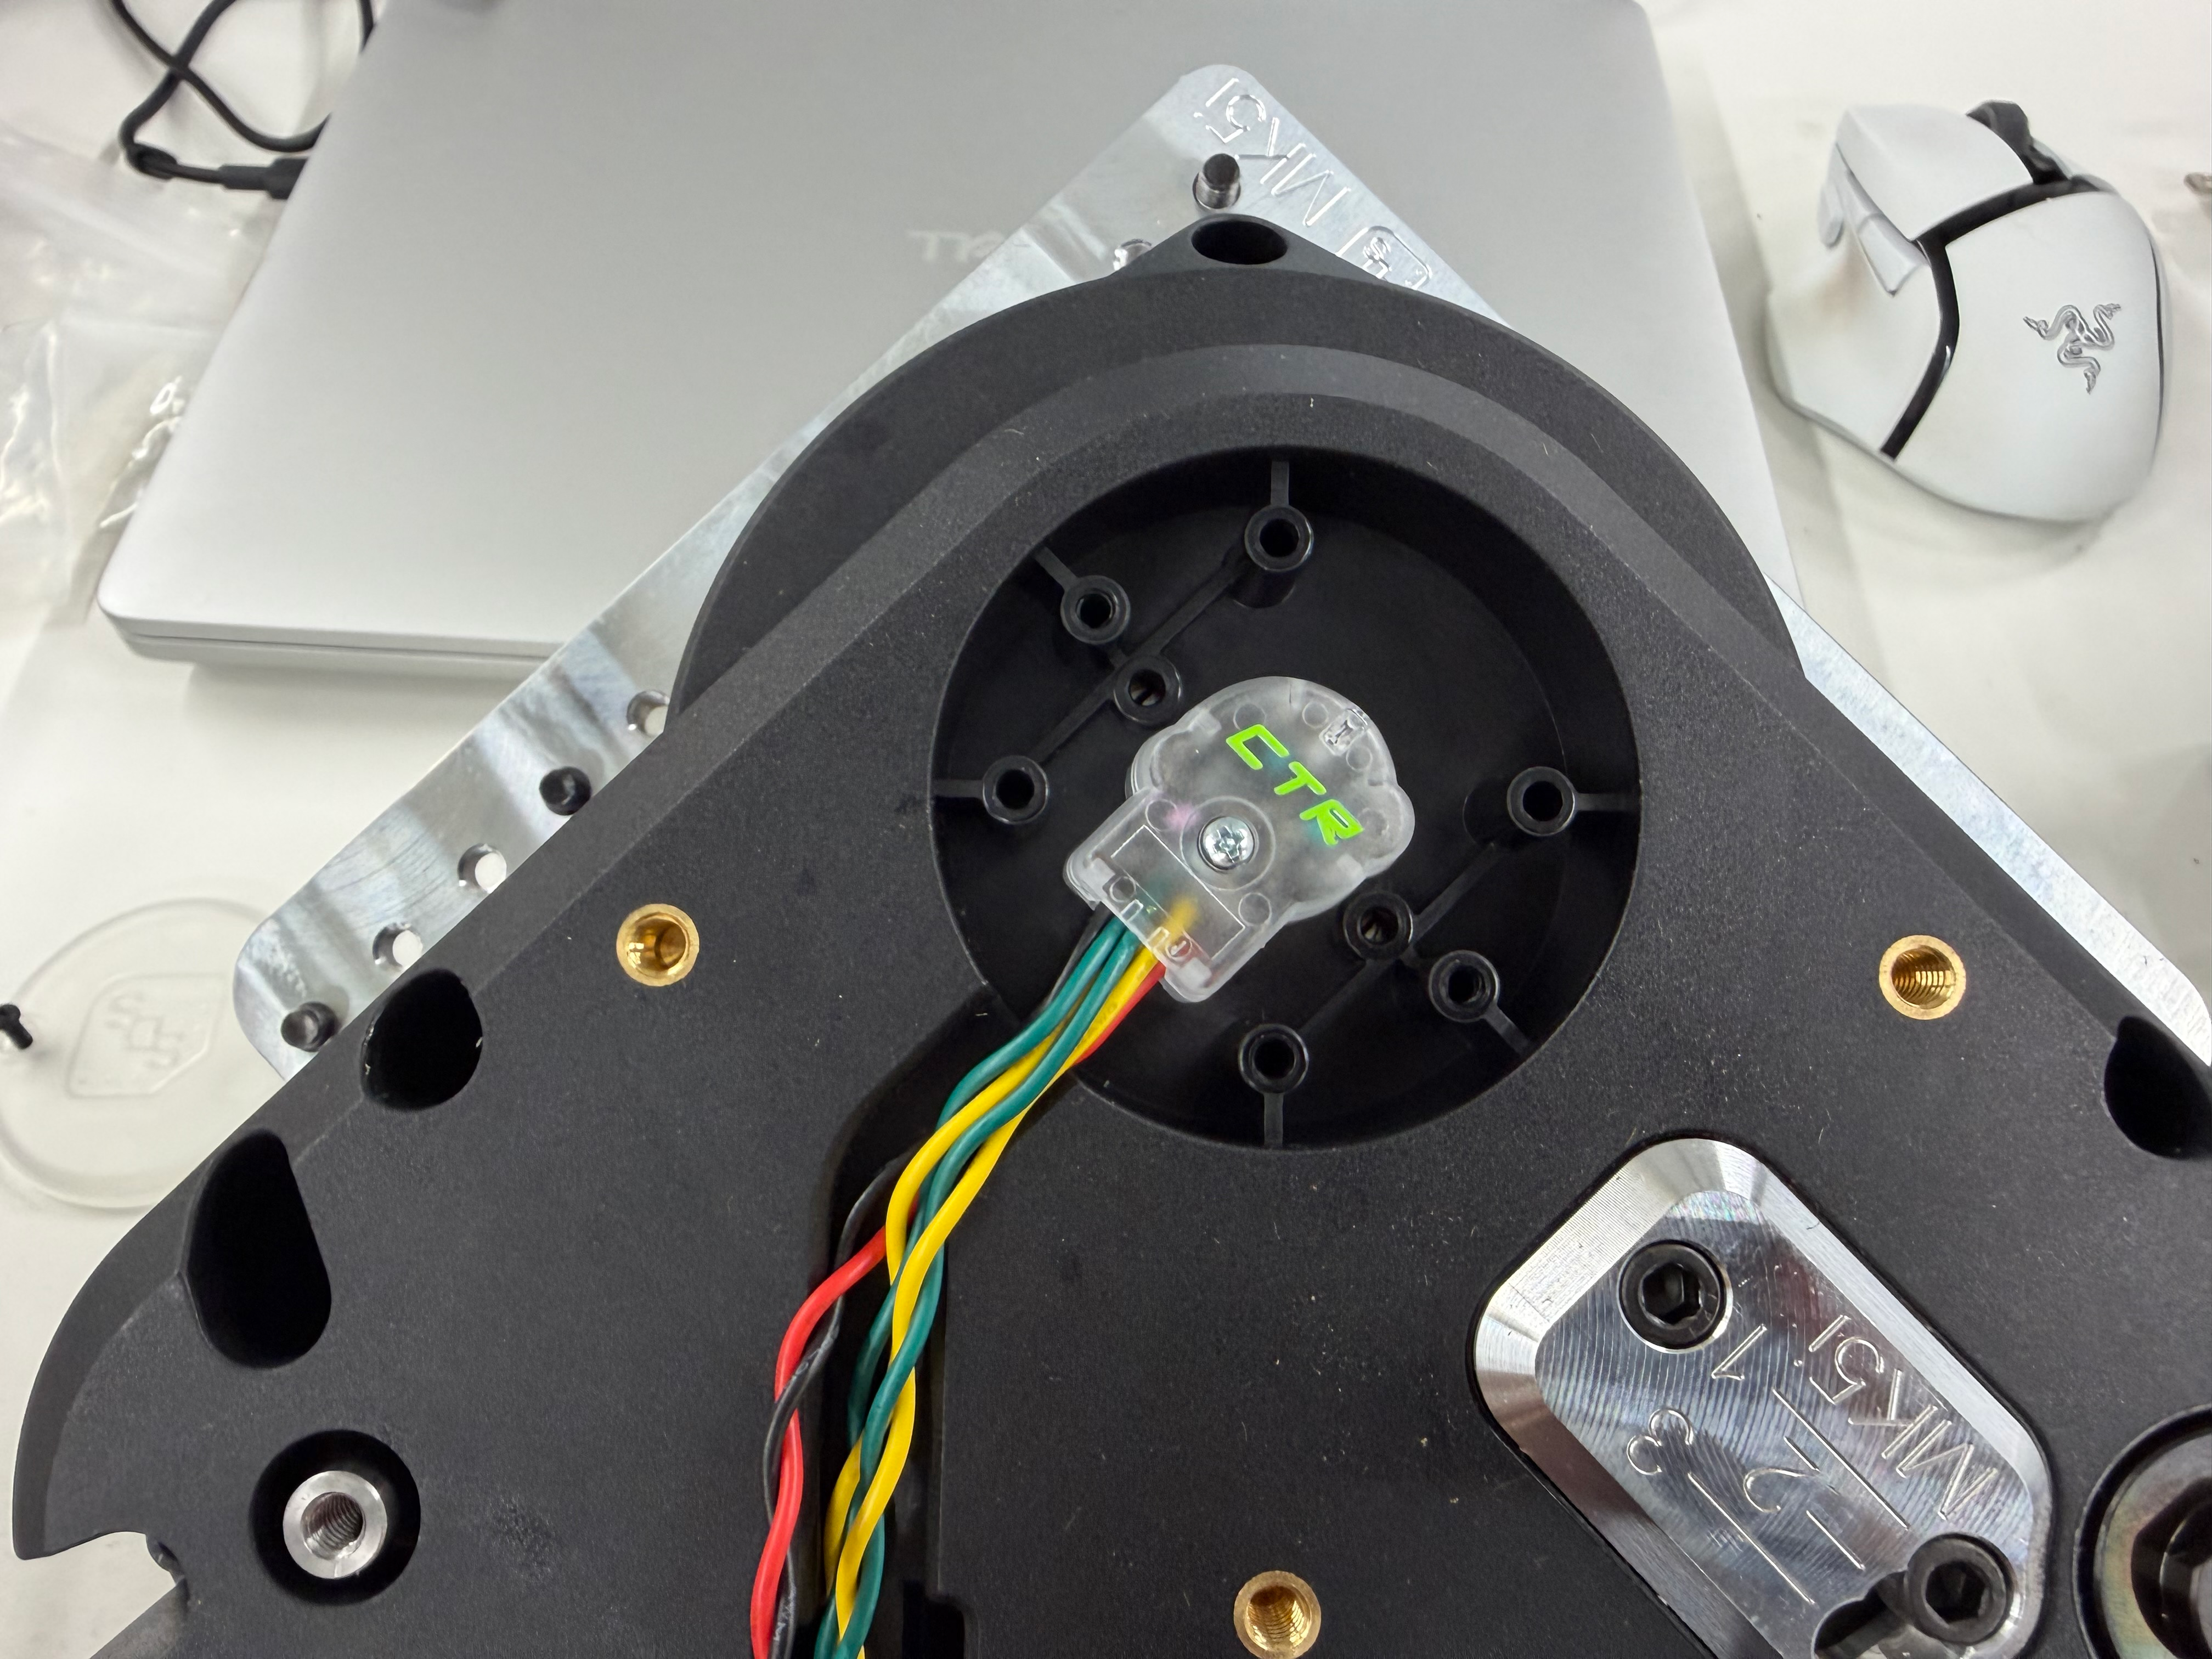
\includegraphics[width=0.31\textwidth]{media/image25.png}
\caption{Seating the encoder between the bottom and top covers, with the
rectangular end toward the wire channel.}
\end{figure}

\assemblystep{Assemble Remaining Modules}
Repeat all steps in this section until you have 4 assembled swerve
modules.
